% !TEX root = ../Dissertation.tex
%===================================================================================================

\chapter{Results}


\section{B cell numbers in the NOD mouse thymus increase with age}

As mentioned previously in \cref{sec:thymicBcells}, it is normal for a small population of B cells, about 0.1-0.5\% of thymocytes, to be present in the thymus of both humans and mice \citep{Perera2013}.
However, it has been noted by our lab (Varian and Green, unpublished observations) and others \citep{OReilly1994}, that this population is significantly increased in the NOD mouse in comparison to a mouse that is not predisposed to T1D, for example, B6 mice.
It is thought that these cells may have a role in the process of T cell negative selection and potentially impede central tolerance of T cells \citep{Starr2003, Perera2013} \toref{Hannahan?}.
For this reason, it is important to establish when and why this thymic abnormality occurs.
%It is not known how thymic B cells come to populate the thymus, however, it is proposed that they either migrate there from the bone marrow, or that they develop within the thymus from progenitors there which have B cell potential \citep{Perera2013}.


It is not clear whether the increased frequency of thymic B cells in NOD mice compared to non-NOD mice is age-related; that is, whether or not the increased population of thymic B cells correlates with a specific stage of the T1D process.
To confirm and extend our previous observations of the increase in thymic B cells in NOD mice compared to control B6 mice, a time-course, flow cytometric study was conducted. %to assess the presence of mature B cells in the thymi of NOD mice and B6 control mice that do not spontaneously develop T1D.
The time points for analysis were chosen to correlate with different stages of the disease process, based on the well defined NOD mouse disease progression (see \cref{fig:diseasecourse}).
As shown in \cref{fig:IncthyBcells}, as NOD mice age and progress along the T1D development pathway, the frequency of mature thymic B cells increases significantly in comparison to control B6 mice. (\cref{fig:IncthyBcells}\ref{subfig:IncthyBcells}), as do the absolute numbers of B cells (\cref{fig:IncthyBcells}\ref{subfig:ThyBcellnumbers}). (Varian and Green, unpublished observations).

Thus, at 4 weeks - the time point in the disease pathway corresponding to priming of the autoreactive T cell repertoire to islet antigens occurs - no differences were seen in either frequencies \cref{fig:IncthyBcells}\ref{subfig:IncthyBcells} or absolute numbers \cref{fig:IncthyBcells}\ref{subfig:ThyBcellnumbers} of mature IgM\textsuperscript{+} B cells in the two strains of mice. 
However, by 9 weeks of age, when insulitis is well established and initial CTL activity to $\beta$ cells is active, there is a significant increase in both the frequency and absolute numbers of thymic B cells in NOD mice with respect to control B6 mice. 
Furthermore, at 12 weeks of age - a time when $\beta$ cell destruction is extensive and initial T1D development is detectable in our colony - this disparity in thymic B cell frequencies between the two strains of mice is even more prevalent.


%It was also necessary to confirm whether or not the NOD mouse has an increased population of B cells overall which could account for the increase in the thymus.
%It is possible that if NOD mice are producing more B cells in the bone marrow as they age, there may be increased migration of B cells to secondary lymphoid organs such as the spleen and lymph nodes, as well as the thymus.
Due to the interesting observation in the thymus, the bone marrow of NOD mice was also investigated to determine if there is a similar age-related increase in B cell frequencies in comparison to cocntrol B6 mice.
To assess this possibility, a time-course, flow cytometric study was carried out to look at the frequencies of B cells in the bone marrow of NOD and B6 mice at the same time points as the thymus time-course study.
As shown in \cref{fig:IncthyBcells}\ref{subfig:BMBcells}, there is no significant difference between the frequency of B cells in the NOD and B6 bone marrow at any age.
Furthermore, no significant difference in B cell frequencies were seen in either spleen or lymph nodes of NOD and B6 mice (Data not shown).
This would suggest that the increase in B cells is specific to the thymus, not to the mouse as a whole.

Finally, to assess whether this increase in thymic B cells impacted on the development of the main T cell subtypes in the thymus, the frequencies of DN, DP and SP T cells in NOD and B6 thymi were compared using flow cytometry.
Analysis of this data, shown in \cref{fig:NODB6Tcells}, revealed that there was no significant difference between NOD and B6 developing T cell populations at any age.

\begin{figure}
	\begin{subfigure}{0.5\textwidth}
	\caption{Thymus}
	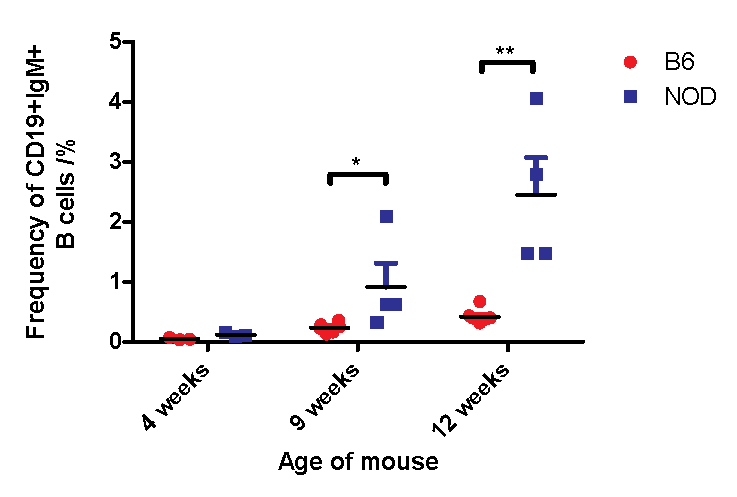
\includegraphics[width=\textwidth]{Figures/IncthyBcells.pdf}	
	\label{subfig:IncthyBcells}
	\end{subfigure}
	\begin{subfigure}{0.5\textwidth}
	\caption{Thymus}
	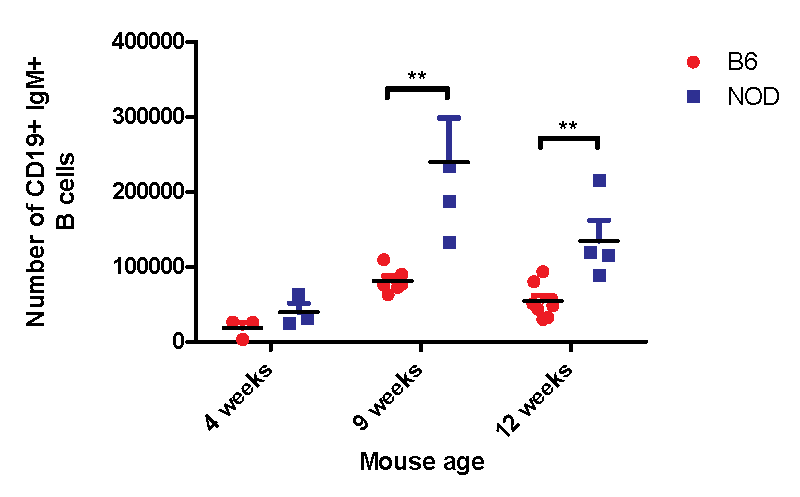
\includegraphics[width=\textwidth]{Figures/ThyBcellnumbers.pdf}
	\label{subfig:ThyBcellnumbers}
	\end{subfigure}
	\begin{subfigure}{0.5\textwidth}
	\caption{Bone Marrow}
	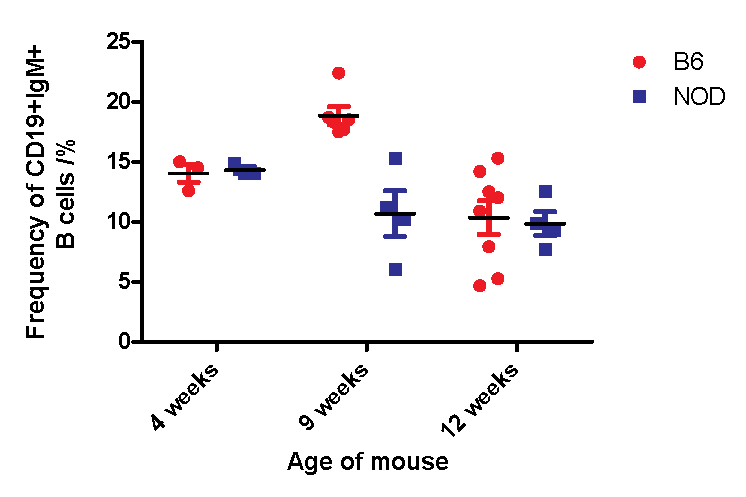
\includegraphics[width=\textwidth]{Figures/BMBcells.pdf}
	\label{subfig:BMBcells}
	\end{subfigure}
\caption[B cell numbers in the NOD mouse thymus increase with age]{B cell numbers in the NOD mouse thymus increase with age. 
Cells were isolated from the above tissues, incubated with anti-CD19 and IgM antibodies and the frequencies (\ref{subfig:IncthyBcells}, \ref{subfig:BMBcells}) and absolute numbers (\ref{subfig:ThyBcellnumbers}) of IgM\textsuperscript{+}CD19\textsuperscript{+} mature B cells in a live, single cell gate, was determined by flow cytometry.
Statistical significance in B cell populations between NOD and B6 mice was determined using the Mann Whitney non-parametric test.

Frequency \ref{subfig:IncthyBcells} and absolute number \ref{subfig:ThyBcellnumbers} of B cells is significantly increased in the NOD thymus, but not bone marrow \ref{subfig:BMBcells} compared to B6 controls.
\ref{subfig:IncthyBcells} and \ref{subfig:ThyBcellnumbers} show the frequency and numbers of B cells in the NOD and B6 thymus, whereas \ref{subfig:BMBcells} shows the frequency of B cells in the NOD and B6 bone marrow.
Data gated lymphocytes, single cells then mature B cells were identified based on the expression of CD19 and IgM.
The Mann Whitney test was used to compare the difference in mature B cell frequency at each age. Differences between NOD and B6 were statistically significant at both 9 and 12 weeks of age (P=0.0190 and P=0.0040, respectively). The difference at 4 weeks is not statistically significant.
NOD n=3-4, B6 n=3-6.}
\label{fig:IncthyBcells}
\end{figure}

\begin{figure}
	\begin{subfigure}{0.5\textwidth}
	\caption{}
	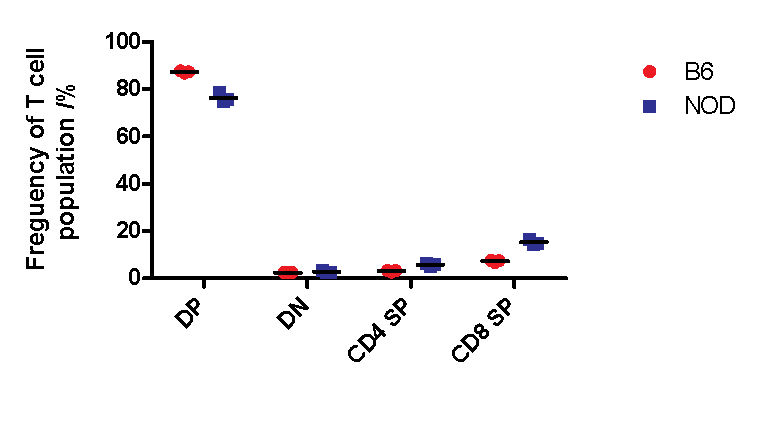
\includegraphics[width=\textwidth]{Figures/4wkThyTcells.pdf}
	\label{subfig:4wkThyTcells}
	\end{subfigure}
	\begin{subfigure}{0.5\textwidth}
	\caption{}
 	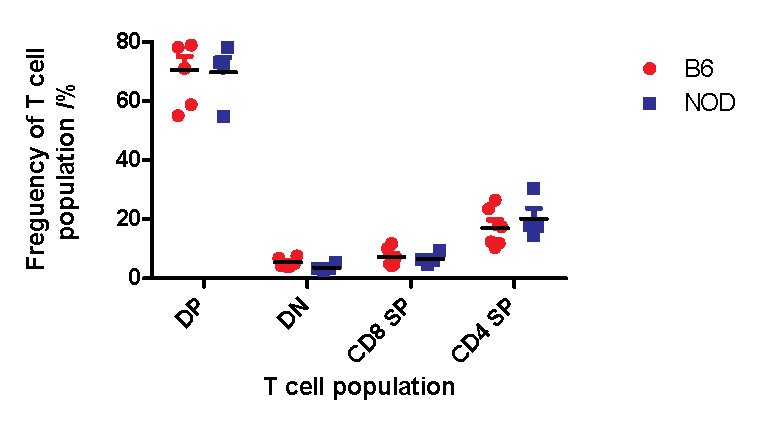
\includegraphics[width=\textwidth]{Figures/9wkThyTcells.pdf}
	\label{subfig:9wkThyTcells}
	\end{subfigure}
	\begin{subfigure}{0.5\textwidth}
	\centering
	\caption{}
 	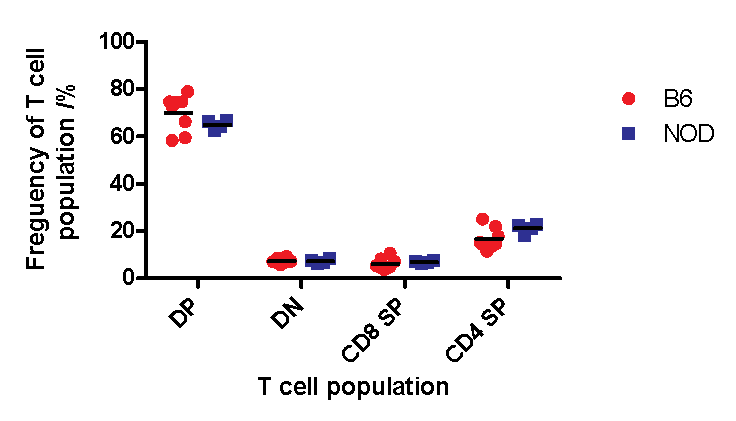
\includegraphics[width=\textwidth]{Figures/12wkThyTcells.pdf}
	\label{subfig:12wkThyTcells}
	\end{subfigure}
\caption[T cell development is normal in the NOD mouse]{T cell populations are normal between NOD and B6. \ref{subfig:4wkThyTcells} 4 weeks, \ref{subfig:9wkThyTcells} 9 weeks, \ref{subfig:12wkThyTcells} 12 weeks.}
\label{fig:NODB6Tcells}
\end{figure}


\subsection{The NOD thymus contains B cell development transcription factors}
\label{subsec:TFs}

12 wks old

If B cells are developing within the thymus, this begs the question as to whether the NOD thymus is providing an environment conducive to B cell development. 
\todo{few sentences of rationale of why I selected these TFs, reminder from intro}
To investigate this, primers were designed that were specific for B cell development factors such as E2A, EBF, Pax5, VPreB and CXCL12.
These primers were chosen as they are important for lineage commitment and/or lineage progession and stabilisation.
E2A is important for the formation of pro B cells and is a requirement for the expression of EBF.
EBF is then important for activating genes and transcription factors crucial for BcR rearrangement, such as VPreB and FOXO1.
Pax5 is important for the progression of progenitors within the B cell lineage and for the repression of transcription factors driving development of other lineages, for example, Notch1 for T cell development.
CXCL12 is a cytokine responsible for holding B cell progenitors in the bone marrow niche during development.
%\todo{look in Hagman2006, Welinder2011, Mansson2008, Cobaleda2007, Radtke2013, Riley2013, Tokoyoda2004 for TF info}.

Non-quantitative RT-PCR was performed to compare whether or not B cell development genes and transcription factors are present in the thymus of 11-12 week old NOD mice.
The bone marrow was included as a control tissue since this is the normal site of B cell development.
All transcription factors would be expected to be detectable in the bone marrow and this was the case, as shown in \cref{fig:gels}.
Interestingly, all the genes, besides CXCL12 (\cref{fig:gels}\ref{subfig:CXCL12}), were also present in the NOD thymus too.
This reinforces the idea that the thymic environment is able to support and/or promote B cell development.
The lack of CXCL12 in the thymus is not a surprising result as it is a cytokine responsible for holding developing B cells in the bone marrow niche and therefore, may be more bone marrow specific rather than B cell specific.
This raises the question as to what chemokine is holding developing B cells in the thymic niche to enable completion of their development if it isn't CXCL12.

It would be beneficial to carry out quantitiative PCR to determine relative expression levels between the bone marrow and thymus of NOD mice, as non quantitiative PCR can only show presence of a transcription factor.
It would also be useful to compare B6 control mice and NOD mice to see if the thymic environments differed between the diabetes susceptible and non diabetic control mice.
Unfortunately, due to time constraints it was not possible to carry out quantitative PCR for this project.

\begin{figure}
	\begin{subfigure}{0.5\textwidth}
	\centering
	\caption{E2A}
	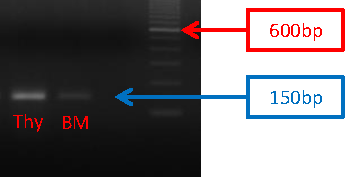
\includegraphics[width=\textwidth]{Figures/E2A.pdf}
	\end{subfigure}
	\begin{subfigure}{0.5\textwidth}
	\centering
	\caption{EBF}
	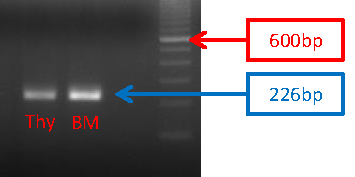
\includegraphics[width=\textwidth]{Figures/EBF.pdf}
	\end{subfigure}
	\begin{subfigure}{0.5\textwidth}
	\centering
	\caption{Pax5}
	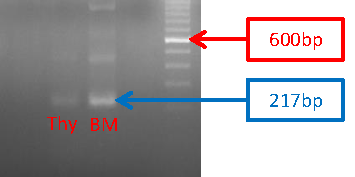
\includegraphics[width=\textwidth]{Figures/sPax5.pdf}
	\end{subfigure}
	\begin{subfigure}{0.5\textwidth}
	\centering
	\caption{VPreB}
	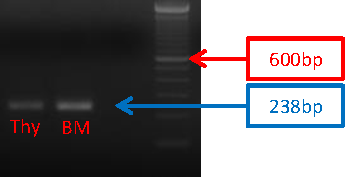
\includegraphics[width=\textwidth]{Figures/VPreB.pdf}
	\end{subfigure}
	\begin{subfigure}{\textwidth}
	\caption{CXCL12}
	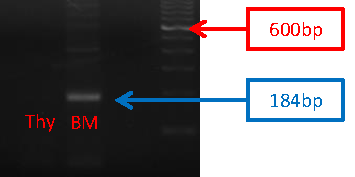
\includegraphics[width=0.5\textwidth]{Figures/CXCL12.pdf}
	\label{subfig:CXCL12}
	\end{subfigure}
\caption[Non quantitative PCR reveals B cell development transcription factors are present in the NOD thymus]{Non quantitative PCR reveals B cell development transcription factors are present in the NOD thymus.
RNA prepared and reverse transcribed to cDNA.
Non-quantitative PCR performed using primers specific for B cell development transcription factors and genes.
Gel electrophoresis carried out to detect PCR product.
Gels were run in 3\% agarose in 1 x TAE buffer. Gels supplemented with 1 $\mu$L ethidium bromide per 25 $\mu$L of 1 x TAE buffer. Gels run at constant 70V.
Lanes from left to right; Thymus, Bone marrow, 100 bp marker. 
600bp mark showed in red box.
Expected product size is shown in blue box.}
\label{fig:gels}
\end{figure}


\subsection{There are pro and pre B cells present in the NOD thymus}
\label{subsec:proandpre}

The mechanism by which B cell frequencies/numbers increase in the NOD thymus is unknown. 
Two potential hypotheses to account for the increase are development from progenitors entering the thymus which have B cell potential, or migration of B cells from the bone marrow. \toref{}
The current consensus is that B cells are developing within the thymus. 

B cells in the bone marrow develop through different developmental stages (See \cref{subsubsec:committedBcelldevelopment}).
The first of these stages is the CD19\textsuperscript{+}CD43\textsuperscript{+}IgM\textsuperscript{-} pro B cell stage.
Subsequently, the IgM heavy chain is rearranged and coupled to a surrogate light chain (such as VPreB), forming the preBCR. \fig{Figure showing b cell development}
The sucessful formation of a preBCR allows progression to the CD19\textsuperscript{+}CD43\textsuperscript{-}IgM\textsuperscript{-} pre B cell stage.
Next, the light chain rearranges resulting in a full IgM molecule and the B cell can be released from the bone marrow to migrate to the spleen to finish its development.

%Pro and pre B cells are seen in normal B cell development in the bone marrow of both NOD and B6 mice, as shown in \cref{subfig:BMpropre}.
%The similarity in the bone marrow between the two strains suggests that B cell development in the bone marrow of the NOD mouse is normal.

\citet{Akashi2000} has shown pro and pre B cells in the thymus of B6 mice.
It is unclear whether similar populations occur in NOD mice, therefore, to determine this, a comparative flow cytometric study was carried out using NOD and B6 mouse thymi.
As a control, the populations of pro and pre B cells in the bone marrow were also assessed, as this is the normal site of B cell development.

As shown in \cref{fig:PropreBcells}\ref{subfig:Thypropre}, pro and pre B cells can be seen in the thymus of NOD and B6 mice.
%Data shown is representative of 3-6 mice aged between 6-9 weeks. %Thymus data HLD 20th July, BM data JV 23.9.09
%This age was chosen as it is the time when mature B cells increase in the thymus of NOD mice compared to B6 mice (\cref{fig:IncthyBcells}\ref{subfig:IncthyBcells}).
The presence of pro and pre B cells suggests that these stages of B cell development may be supported by the thymus. 
%however, it is not possible to say whether these cells have developed in the thymus or migrated there.
%It can only suggest that the thymus is capable of providing an environment where they are able to survive.
As expected, the bone marrow (\cref{fig:PropreBcells}\ref{subfig:BMpropre}) also shows populations of pro and pre B cells which appear similar between mouse strains.


%Presence of these developing B cells suggest that B cells could be developing within the thymus and that further investigation is warranted.}



\begin{figure}	
	\begin{subfigure}{\textwidth}
	\centering
	\caption{Thymus}
	\includegraphics[width=0.7\textwidth]{Figures/Thymuspropre.png}
	\label{subfig:Thypropre}
	\end{subfigure}
	\begin{subfigure}{\textwidth}
	\centering
	\caption{Bone marrow}
	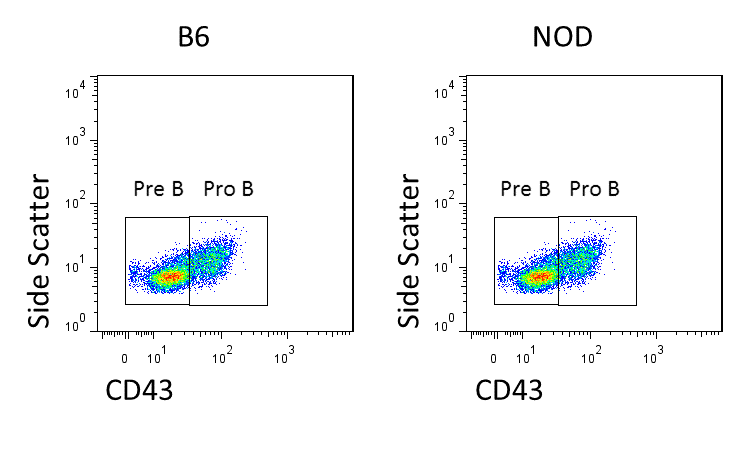
\includegraphics[width=0.7\textwidth]{Figures/Bonemarrowpropre.png}
	\label{subfig:BMpropre}
	\end{subfigure}
\caption[Pro and pre B cells are present in NOD and B6 thymi]{Pro and pre B cells are found in the thymus (\ref{subfig:Thypropre}) and bone marrow (\ref{subfig:BMpropre}) of both NOD and B6 mice. Single cell suspensions were prepared and incubated with anti-CD19, -IgM and -CD43 antibodies. 
Pro (CD19\textsuperscript{+}IgM\textsuperscript{-}CD43\textsuperscript{+}) and pre (CD19\textsuperscript{+}IgM\textsuperscript{-}CD43\textsuperscript{-}) B cells within a live, single cell gate were identified by flow cytometry.
For the thymus, the cells were acquired on a CD19\textsuperscript{+} gate to enrich for B cells. 
The data shown is representative of 

For analysis, samples were gated lymphocytes, single cells, CD19\textsuperscript{+}, IgM\textsuperscript{-} then split into pro and pre B cells using CD43 expression. Bone marrow plots are representative of 4 NOD and 6 B6 mice. Thymus plots are representative of 3 NOD and 4 B6 mice. All mice are aged between 6-9 weeks of age.}
\label{fig:PropreBcells}
\end{figure}





\subsection{Thymic B cell development may be dependent on the presence of a mature B cell}

\todo{Take out B6 data}
The presence of pro and pre B cells in the thymus suggests that thymic B cell development may occur in a similar manner to that occurring in the bone marrow

In the bone marrow, progression from the pro B cell stage to the pre B cell stage requires rearrangement of the IgM heavy chains.
Ablation of IgM heavy chain rearrangement results in blockade of pro to pre B cell stage, and as a consequence an accumulation of pro B cells \toref{Serreze?}.
To assess whether similar pro to pre B cell transition is governed by IgM heavy chain rearrangment in the thymus, comparative flow cytometric analysis of NOD mice with NOD mice that are unable to rearrange the IgM heavy chain (NOD KO mice, \cref{methods:mice}). 

Comparative, flow cytometric studies of NOD and NOD KO bone marrow, as expected, revealed that in NOD KO mice, B cell development was blocked at the pro B cell stage \cref{fig:MatureBincProB} \ref{subfig:KOBM}.
It was therefore expected that in the NOD KO thymus there would also be a population of pro B cells, similar to that seen in the NOD WT mice. 
However, this does not appear to be the case.

When analysing this data, it was important to establish a gating system whereby the two different strains could be compared fairly.
NOD KO mice have no pre B cells and no IgM\textsuperscript{+} cells therefore previous gating to look at pro and pre B cells (CD19\textsuperscript{+} then analysed on IgM and CD43 expression) would be skewed in the NOD KO as 100\% of the cells would be pro B cells, whether or not the population was increased or decreased with respect to the other strains.
With this in mind, IgM\textsuperscript{+} cells were gated out, as were CD43\textsuperscript{-}.
This leaves only IgM\textsuperscript{-}CD43\textsuperscript{+} cells, of which any that are CD19\textsuperscript{+} should be pro B cells.
This means that the frequencies of pro B cells can be compared fairly by the frequency of CD19\textsuperscript{+} cells present within the IgM\textsuperscript{-}CD43\textsuperscript{+} population.
The frequencies of pro B cells in both strains of mice are shown in \cref{fig:MatureBincProB}\ref{subfig:ThyProBcells}.


As shown in \cref{fig:MatureBincProB}\ref{subfig:MatureBincproBgraph}, the frequency of pro B cells in the NOD KO mouse thymus is significantly decreased in comparison to the frequency of pro B cells in the NOD mouse thymus.
This is an interesting finding as it suggests that the enhancement of pro B cells in the thymus may be dependent on the presence of a mature B cell.


\begin{figure}
	\begin{subfigure}{\textwidth}
	\caption{}
	\includegraphics[width=0.7\textwidth]{Figures/NODvKOproBcells.png}
	\label{subfig:ThyProBcells}
	\end{subfigure}
	\begin{subfigure}{\textwidth}
	\caption{}
	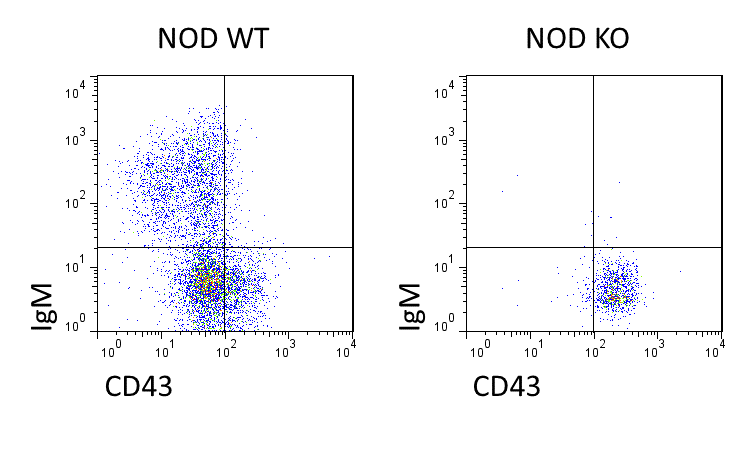
\includegraphics[width=0.7\textwidth]{Figures/NODvKOBM.png}
	\label{subfig:KOBM}
	\end{subfigure}
	\begin{subfigure}{\textwidth}
	\caption{}
	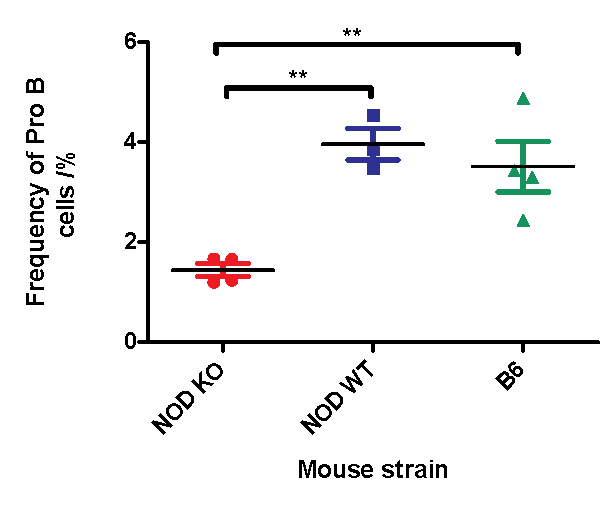
\includegraphics[width=0.5\textwidth]{Figures/MatureBincproBgraph.pdf}
	\label{subfig:MatureBincproBgraph}
	\end{subfigure}
\caption[NOD mice have an increased frequency of pro B cells compared to NOD KO thymi]{Mature B cells increase frequency of pro B cells in the thymus.
Single cell suspensions were prepared from NOD and NOD KO mouse thymi and subsequently incubated with appropriate analytic fluorescent-labelled antibody for flowcytometric analysis.
Samples were gated on acquisition for CD19\textsuperscript{+} cells.
CD19\textsuperscript{+} pro B cells were identified from CD43\textsuperscript{+}IgM\textsuperscript{+} cells in a live, single cell gate.
\ref{subfig:ThyProBcells} shows pro B cells in the thymus of NOD and NOD KO mice.
\ref{subfig:KOBM} shows representative FACS plots of bone marrow from NOD and NOD KO mice.
\ref{subfig:MatureBincproBgraph} is a graphical representation of the frequency of pro B cells in the NOD and NOD KO thymi. Statistical significance determined using the Mann Whitney test. todoSignificance. P<0.05 deemed significant, P=?.
NOD n=3, NOD KO n=4. Mice all aged 6-8 weeks. Experiment was carried out single blind to avoid bias.}
\label{fig:MatureBincProB}
\end{figure}


%\subsection{NOD mice express higher levels of CD43 in the thymus}
%\label{Results:CD43}

%During analysis of the data showing pro B cell presence in the NOD thymus, it was noted that there were differences in CD43 expression between mice of NOD background and B6 controls.
%CD43 is thought to be involved in T cell activation and adhesion in vitro \citep{McEvoy1997} and T cell migration from the blood into lymphoid tissues in vivo \citep{Johnson1999}.
%Further to this, it seems that an anti-CD43 antibody is capable of preventing T1D in NOD mice \citep{Johnson1999}, suggesting that it may have a role in T1D pathogenesis.
%Given the potential implication of CD43 in T1D pathogenesis, the discrepancy in CD43 expression was investigated.

%Samples were gated on lymphocytes, single cells and IgM\textsuperscript{-} cells.
%The frequency of IgM\textsuperscript{-} cells in the thymus was very similar between all mouse strains, however, CD43 expression appeared to be increased in NOD and NOD KO compared to B6, as shown in \cref{fig:CD43expression}.
%Statistical analysis shows that the difference in frequencies of IgM\textsuperscript{-}CD43\textsuperscript{+} between the NOD KO and B6 is statistically significant \todo{P values, check stats}.
%However, there appears to be a wide spread of frequencies of IgM\textsuperscript{-}CD43\textsuperscript{+} cells in both NOD and NOD KO mice.
%This suggests that the experiments need to be repeated to try and increase the reproducibility of the results.
%This spread is not seen in the B6 mouse suggesting that the thymic environment of the B6 mouse may be more regulated than the NOD which shows varying frequencies of IgM\textsuperscript{-}CD43\textsuperscript{+} cells.


%\begin{figure}
	%\begin{subfigure}{\textwidth}
	%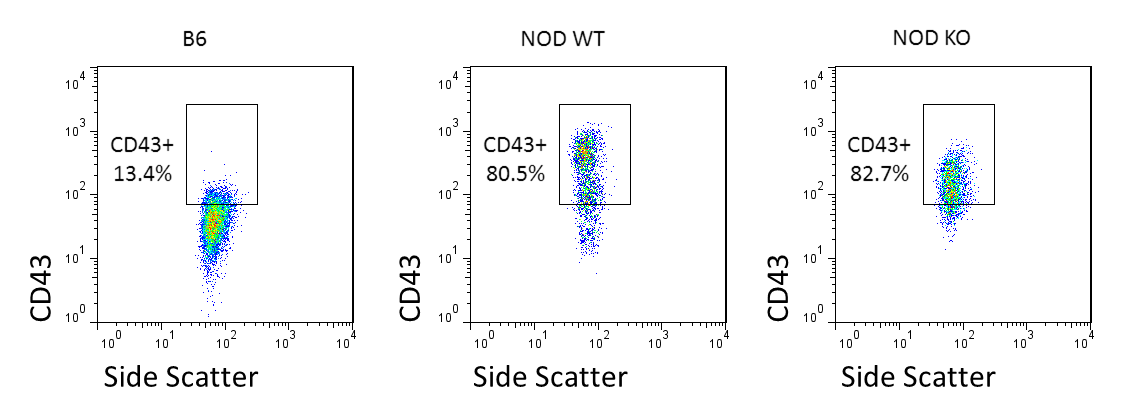
\includegraphics[width=\textwidth]{Figures/CD43expression.png}
	%\caption{Figure showing CD43 expression in IgM- cells in the thymus}
	%\end{subfigure}
	%\begin{subfigure}{\textwidth}
	%\centering
	%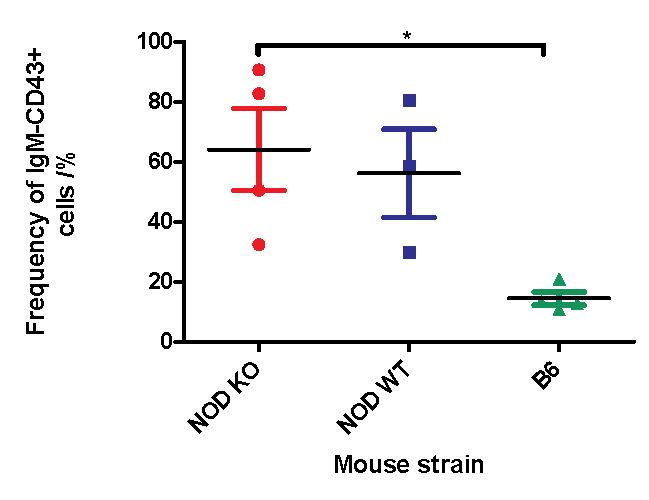
\includegraphics[width=0.6\textwidth]{Figures/CD43levels.pdf}
	%\caption{Graph showing increased CD43 expression NOD}
	%\end{subfigure}
%\caption[Mouse of the NOD background have higher levels of CD43 expression compared to B6]{NOD mice show increased CD43 expression in the thymus.
%Top panel shows representative FACS plots showing increased CD43 expression in NOD WT and NOD KO mice.
%However, the graph shows that the difference is only significant between the NOD KO and B6, analysed using a One-Way ANOVA and Tukey's test.
%FACS plots gated lymphocytes, single cells, IgM\textsuperscript{-} then analysed on CD43 expression.
%NOD KO n=4, NOD WT n=3, B6 n=4. 
%Experiment carried out single blind.}
%\label{fig:CD43expression}
%\end{figure}

%CD43 levels on B cells from last year???

\subsection{Mature NOD thymic B cells are killed following transfer into NOD KO recipients}

The finding that the frequency of pro B cells was decreased in NOD KO mice with respect to NOD mice (\cref{fig:MatureBincProB}), suggested thymic B cell development was dependent on the presence of a mature B cell, potentially one that resided within the thymus itself.
In order to investigate the role of thymic B cells in the future, and determine whether or not they have an effect on the pro B cell population seen in the thymus, as suggested above, a suitable experimental approach would need to be decided upon first.
A potential approach would be to transfer mature thymic B cells from NOD donors into NOD KO recipients.
A similar approach has been tried by \citet{Serreze1998} which resulted in CTL destruction of the transferred B cells, suggesting that this approach may not work.
However, \citet{Serreze1998} transferred splenic B cells rather than thymic B cells and since the properties of thymic B cells are not well understood, it may be that the same thing does not occur.
%The finding that the frequency of pro B cells was decreased in NOD KO mice with respect to NOD mice suggests that a mature B cell might have an impact on the development or survival of thymic pro B cells.

To investigate this, a pilot study was performed whereby thymic cells, including thymic B cells, were isolated from NOD mice and transferred into NOD KO mice, to see whether they could survive in the NOD KO recipients.

Due to the preliminary nature of the transfer experiment, very small numbers of mice were used.
10 week old female donor NOD and recipient NOD KO mice were used.
Thymic B cells are significantly increased in NOD mice of this age compared to control B6 mice therefore this time point was chosen.
%Also, the frequencies/numbers are still increasing at this age in comparison to control B6 mice therefore any mechanisms increasing thymic B cells should be active at this age.
The experimental set up for this transfer experiment is shown in \cref{fig:Transfersetup}\ref{fig:KOtransfersetup}.
Thymocytes were prepared from two donor mice and the CD19\textsuperscript{+} and CD19\textsuperscript{-} populations were separated using magnetic assisted cell sorting. 
Purity of the cell populations was determined by cytometry (see \cref{fig:Transfersetup}\ref{subfig:NODdonorseparation}) and the two cell populations were injected into appropriated labelled NOD KO recipients.
The recipient mice were assessed at 7 days and 11 days following transfer of donor cells to determine the initial and long term population of various tissues with mature B cells.
Both primary (thymus and bone marrow) and secondary (spleen, pancreatic and axillary lymph nodes) were assessed.



The aim of the transfer was to see if the medthodology would be appropriate for examining the role of thymic B cells, therefore it was important to have a donor fraction that contained thymic B cells and a control donor population that did not.
The aim of the separation was to have a fraction that contained no B cells (CD19\textsuperscript{-} fraction), and a fraction that contained thymic B cells (CD19\textsuperscript{+} fraction) so that in future experiments, any effects of thymic B cells in the recipients could be identified.

The donor thymi were taken from the donor mice and split into CD19\textsuperscript{+} and CD19\textsuperscript{-} fractions using CD19 microbeads (Miltenyi).
Flow cytometric analysis of the separated donor thymi fractions are shown in \cref{fig:Transfersetup}\ref{subfig:NODdonorseparation}. %and \cref{subfig:GFPdonorseparation}.
The separations worked well in that the CD19\textsuperscript{-} fractions had very few contaminating B cells (See \cref{fig:Transfersetup}\ref{subfig:NODdonorseparation}).
The CD19\textsuperscript{+} fractions contain almost 100\% of thymic B cells, however, they are contaminated with non B cells.
With this in mind, the separation worked as there were very few B cells present in the CD19\textsuperscript{-} fraction compared to the CD19\textsuperscript{+} fraction.


\begin{figure}
	\begin{subfigure}{\textwidth}
	\centering
	\caption{}
	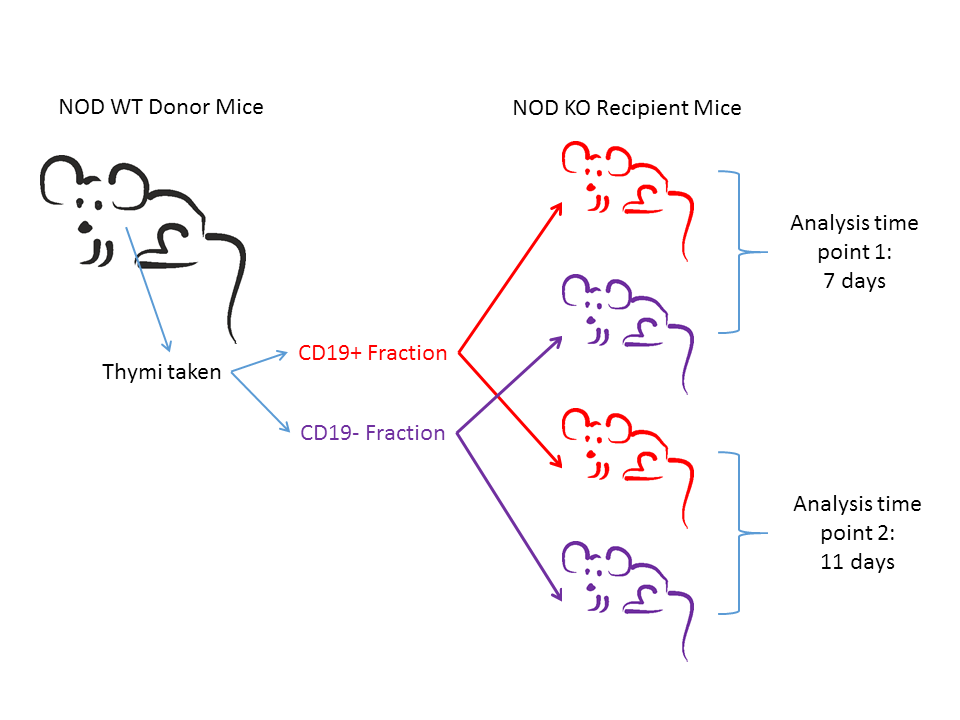
\includegraphics[width=0.7\textwidth]{Figures/KOTransferexptsetup.png}
	\label{fig:KOtransfersetup}
	\end{subfigure}
	\begin{subfigure}{0.5\textwidth}
	\caption{}
	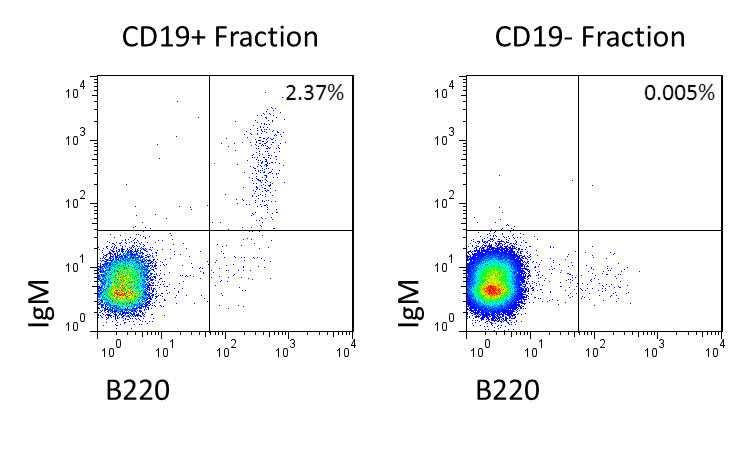
\includegraphics[width=\textwidth]{Figures/NODdonor.png}
	\label{subfig:NODdonorseparation}
	\end{subfigure}
	\begin{subfigure}{0.5\textwidth}
	\centering
	\caption{}
	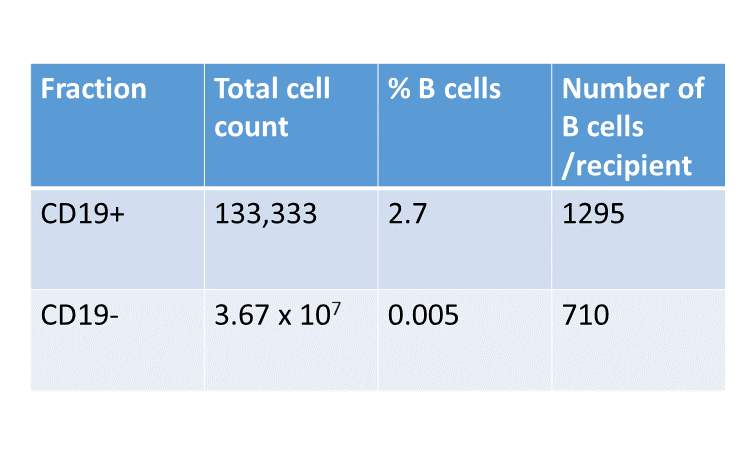
\includegraphics[width=\textwidth]{Figures/WTdonortable2.png}
	\label{subfig:WTdonortable}
	\end{subfigure}
\caption[Experimental setup and donor cell populations for transfer experiments]{}
\label{fig:Transfersetup}
\end{figure}
	
	
The donor populations were transferred by intravenous injection into the recipient mice then the recipient tissues were analysed by flow cytometry at the stated time points.
As shown in figure \cref{fig:Transfer}, flow cytometric analysis revealed that mature B cells (CD19\textsuperscript{+}IgM\textsuperscript{+}) were only present in the recipient mice at the 7 day post transfer time point.
The inability to detect mature B cells at the later, 11 day timepoint, may reflect cytotoxic killing of these cells in NOD KO mice \citep{Serreze1998}.
At either time point, no mature B cells were detectable in the bone marrow or any lymph node analysed (Data not shown).
In contrast, both the spleen \cref{fig:Transfer}\ref{subfig:transferspleen} and thymus \cref{fig:Transfer}\ref{subfig:transferthymus} of NOD KO mice contained mature B cells at the 7 day time point.
%On the other hand, due to the fact that the group size is very small (one mouse per group), the results must be viewed with caution.


Although B cells are seen in the thymus and spleen of both recipients at the 7 day time point, it seems that there is a higher frequency of CD19\textsuperscript{+}IgM\textsuperscript{+} cells in the recipients that received the CD19\textsuperscript{+} cell containing donor cells.
This finding is not surprising as this recipient received more mature B cells in the transferred cells.

In the CD19\textsuperscript{-} recipients, there are also mature B cells present in the spleen and thymus at the 7 day time point.
The population in the spleen could reflect contaminating B cells which were transferred. 
It is unlikely that these B cells seen have developed from CD19\textsuperscript{-} progenitors due to B cells not normally developing in the spleen.
However, while the population of B cells in the thymus could also be due to contaminating transferred B cells, it may be that within the thymus, there is the potential for CD19\textsuperscript{-} B cell progenitors to develop into mature B cells there.
%However, there are still some B cells seen in the CD19\textsuperscript{-} recipient.
%These could be B cells that developed from CD19\textsuperscript{-} progenitors which were injected or they may be contaminating B cells that were transferred.


The aim of the experiment was to look at the lifespan of B cells following transfer into recipient NOD KO mice, to see if this would be a viable method for investigating the effect of mature B cells of thymic pro B cell frequency.
However, it has shown that this methodology is not appropriate for these investigations due to the disappearance of transferred cells between 7 and 11 days post transfer.
Although the reason for their disappearance is not clear, it may be that CTLs are destroying thymic B cells, similarly to the CTL destruction of splenic B cells seen by \citet{Serreze1998}

\begin{figure}
	\begin{subfigure}{\textwidth}
	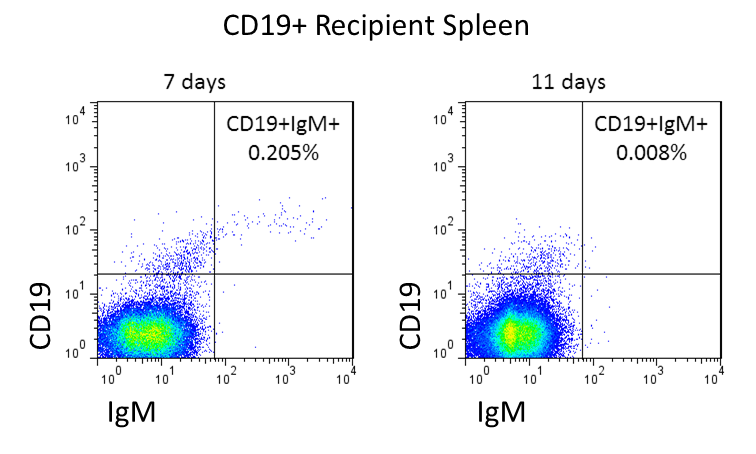
\includegraphics[width=0.5\textwidth]{Figures/CD19posrecipspleen.png}
	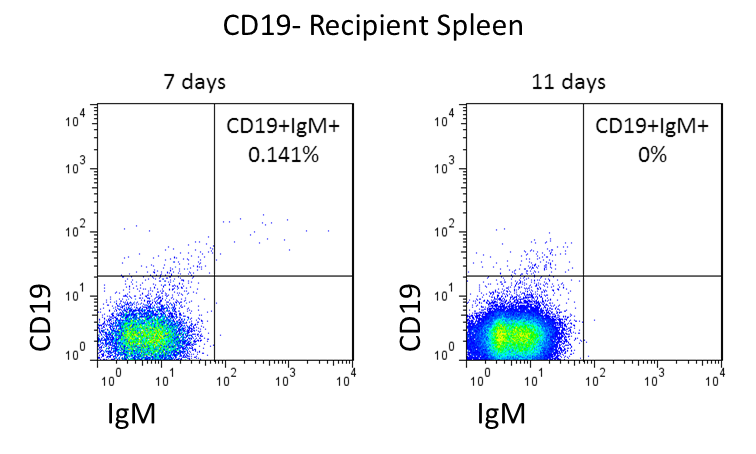
\includegraphics[width=0.5\textwidth]{Figures/CD19negrecipspleen.png}
	\caption{Spleen of recipient mice showing frequency of CD19+IgM+ B cells at 7 and 11 days post transfer}
	\label{subfig:transferspleen}
	\end{subfigure}
	\begin{subfigure}{\textwidth}
	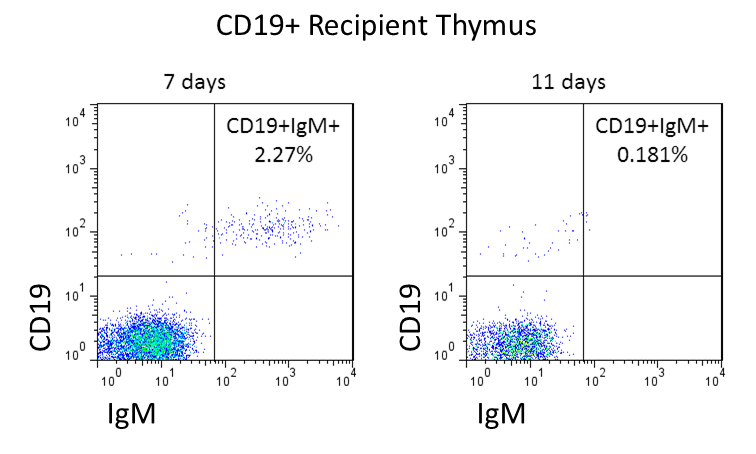
\includegraphics[width=0.5\textwidth]{Figures/CD19posrecipthy.png}
	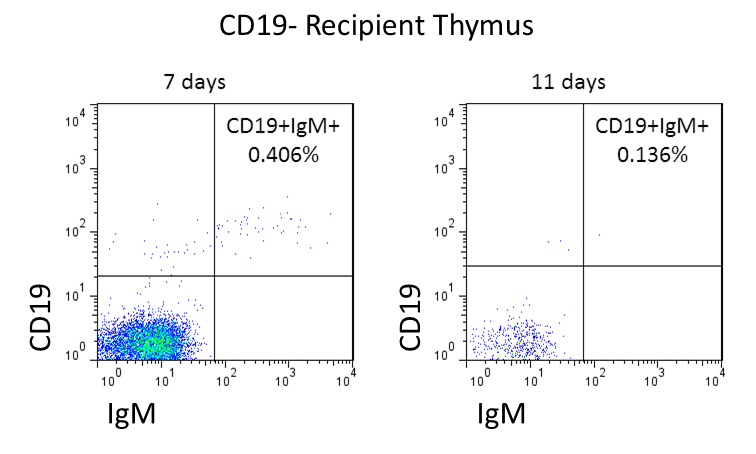
\includegraphics[width=0.5\textwidth]{Figures/CD19negrecipthy.png}
	\caption{Thymus of recipients showing B cell presence/absence at 7 and 11 days post transfer}
	\label{subfig:transferthymus}
	\end{subfigure}
\caption[Donor B cells are found in the spleen of recipient mice at 4 days post transplant]{Figure showing B cell presence/absence in spleen and thymus over time.
Top panel shows B cell presence in the spleen of the CD19+ and CD19- recipients at 7 and 11 days post transfer.
Bottom panel shows the same but in the recipient thymi.
Data shown is gated lymphocytes, single cells, GFP\textsuperscript{+} then analysed on CD19 expression.
n=1 for every group.
The experiment was carried out double blind to avoid bias during analysis.}
\label{fig:Transfer}
\end{figure}

%It was then wondered whether or not the recipient NOD KO mice had an increase in pro B cells in the thymus due to the effect of transferred B cells.
%However, it appears that there is no difference in the frequency of pro B cells between the KO control and either recipient (Data not shown).
%The results were also very varied and inconsistent therefore the group sizes would need to be increased significantly and the experiment repeated in order to obtain any meaningful results.




\subsection{The NOD thymus can support BcR rearrangement}

Initial rearrangement of the BcR takes place at the pro to pre B cell transition phase, and the finding that pre B cells are present in the NOD thymus suggests that the thymus can support early rearrangments of the BcR.
To confirm this, NOD-RAG-GFP reporter mice were utilised to look for RAG expression by developing thymic B cells.
If RAG is being expressed by CD19\textsuperscript{+} cells in the thymus, this is definitive evidence that B cells are developing in the thymus, rather than just relying on seeing cells with the phenotypes of pro and pre B cells.

NOD-RAG-GFP reporter mice express GFP under the control of the RAG promoter, therefore, during receptor rearrangement when RAG is being transcribed, GFP is also produced and can act as a marker for RAG activity.
Further to this, while transcription of RAG and GFP cease simultaneously, GFP degrades slowly over time with a half life of approximately 56 hours in vivo \citep{McCaughtry2007}.
This means that the intensity of GFP signal seen on flow cytometry correlates with how recently RAG/GFP transcription was active.
For example, as shown in \cref{subfig:BMRAG} the GFP\textsuperscript{high} population in the bone marrow represents the developing B cells which are actively rearranging their receptor.
The GFP\textsuperscript{low} population shows the cells that have recently rearranged their receptor and subsequently deactivated RAG/GFP transcription, therefore, the GFP signal is decreased.
The GFP\textsuperscript{-} population represents cells which rearranged their receptor more than 56 hours previously.

Murine strains of RAG-GFP reporter mice have been invaluable at documenting the differing frequencies of developing, newly developed and long term resident thymic T regulatory cells depending on co-stimulatory signals \citep{Cuss2012}.
Thus, NOD-RAG-GFP mice enabled analysis not only of BcR rearrangment in developing B cell populations, but also the proportion of developing, newly developed and long term resident thymic B cells.

To investigate whether the thymus may be able to support BcR rearrangement, depending on the stage of the disease, cells of the B cell lineage were identified by expression of CD19 then these cells were interrogated for their GFP expression.
As shown in \cref{fig:GFP}\ref{subfig:RAGhighlownegthyB}, there are CD19\textsuperscript{+}GFP\textsuperscript{high} cells within the thymus of NOD mice at 4, 7 and 11 weeks of age.
This finding confirms that the NOD thymus supports rearrangment of the NOD BcR, as no CD19\textsuperscript{+}GFP\textsuperscript{+} cells would be detectable if it did not.
%This finding suggests that these B cells are actively rearranging their receptor in the thymus.
%If these cells had migrated to the thymus from the bone marrow, it would be expected that the GFP expression would be lower due to GFP decay during the migration process.
Further to this, as shown in \cref{subfig:RAGhighlowneggraph}, interestingly, it appears that the frequency of CD19\textsuperscript{+}GFP\textsuperscript{+} cells decreases as mice progress through the T1D process.
In particular, the frequency of CD19\textsuperscript{+}GFP\textsuperscript{low} cells decreases significantly between 4 and 11 weeks of age.
Conversely, the frequency of the CD19\textsuperscript{+}GFP\textsuperscript{-} increases significantly between 4 and 7 weeks of age.
The significant decrease in CD19\textsuperscript{+}GFP\textsuperscript{low} cells in the NOD thymus could show that there is a decreased frequency of newly developed B cells in the thymus of older NOD mice.
This could be due to a decrease in B cell development, or increased emigration of newly developed B cells.
This is an interesting result as it could suggest that the support of early BcR rearrangement in the thymus is limited to younger mice.



\begin{figure}
	\begin{subfigure}{\textwidth}
	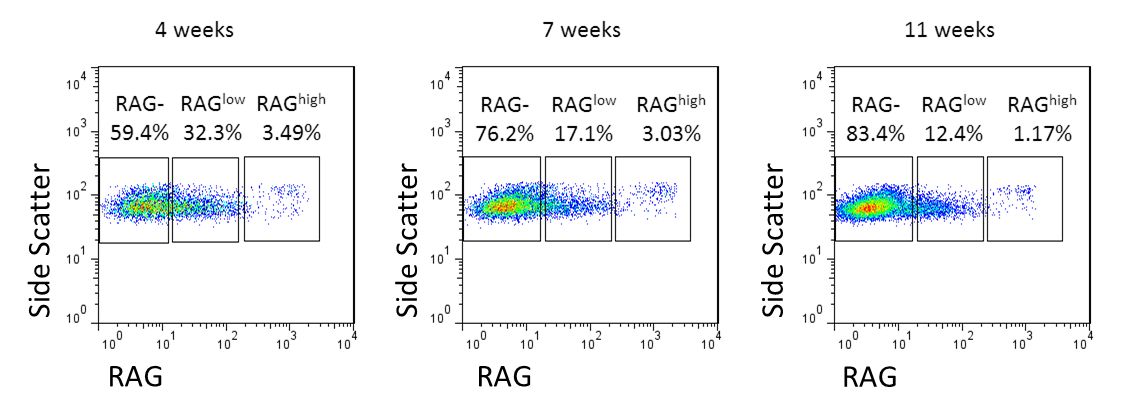
\includegraphics[width=\textwidth]{Figures/RAGhighlownegthyB.png}
	\caption{}
	\label{subfig:RAGhighlownegthyB}
	\end{subfigure}
	\begin{subfigure}{0.5\textwidth}
	\centering
	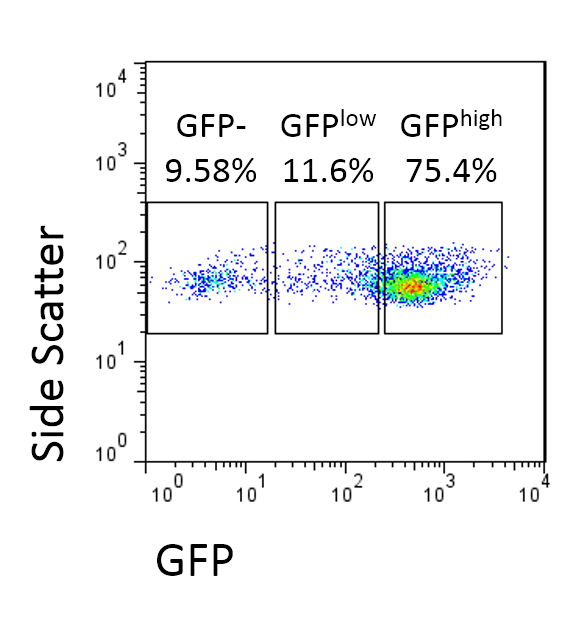
\includegraphics[width=0.7\textwidth]{Figures/7wkBMRAG.png}
	\caption{}
	\label{subfig:BMRAG}
	\end{subfigure}
	\begin{subfigure}{0.5\textwidth}
	\centering
	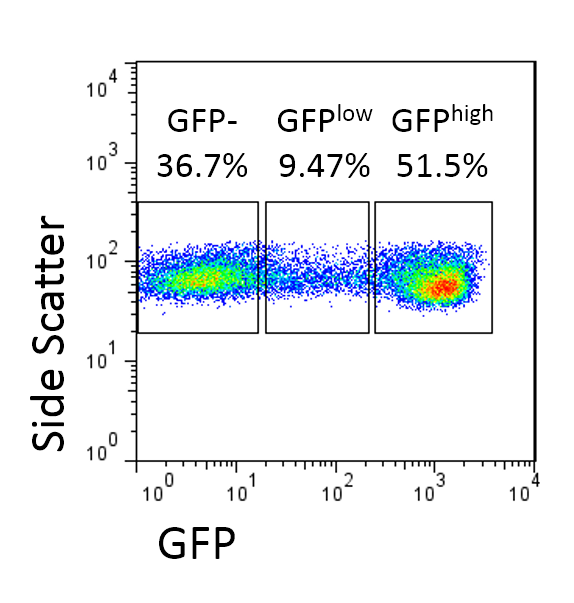
\includegraphics[width=0.7\textwidth]{Figures/7wktotalthyRAG.png}
	\caption{}
	\label{subfig:totalthyRAG}
	\end{subfigure}
	\begin{subfigure}{\textwidth}
	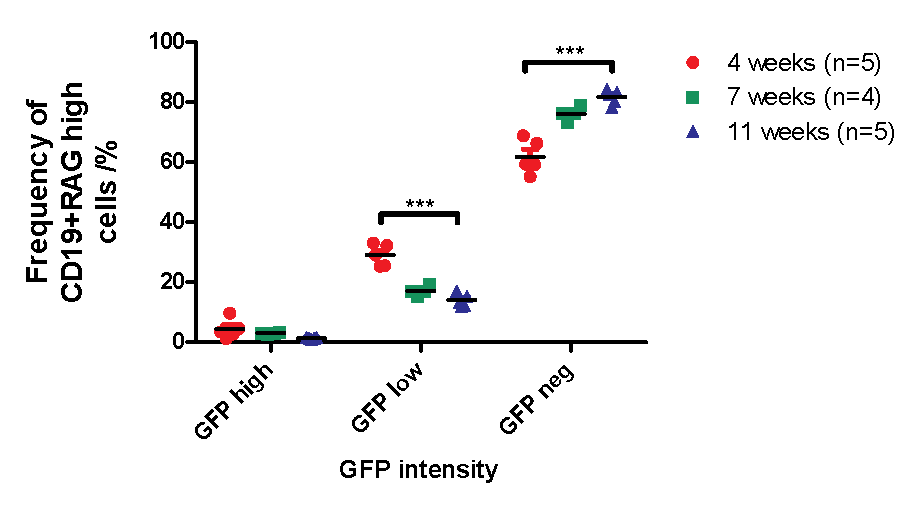
\includegraphics[width=\textwidth]{Figures/RAGhighlownegative.pdf}
	\caption{}
	\label{subfig:RAGhighlowneggraph}
	\end{subfigure}
\caption[Some CD19\textsuperscript{+} cells in the thymus appear to be expressing RAG]{CD19\textsuperscript{+} cells in the NOD thymus express RAG. 
(a) shows the RAG expression of CD19+ cells in the thymus of NOD-RAG-GFP reporter mice at 4, 7 and 11 weeks of age. Each plot is representative of 4/5 sex-matched mice of given age. Single cell suspensions prepared then stained for flow cytometry. Samples gated on acquisition for CD19\textsuperscript{+} cells. For analysis, samples gated lymphocytes, single cells, CD19\textsuperscript{+}. (b) shows RAG expression in the NOD bone marrow, gated lymphocytes, single cells, CD19\textsuperscript{+}. Data representative several mice. (c) shows the total thymic RAG expression used to set gates of RAG\textsuperscript{high}, RAG\textsuperscript{low} and RAG-. Data gated on lymphocytes and single cells. (d) is a graph showing the change in frequency of RAG\textsuperscript{high}, RAG\textsuperscript{low} and RAG\textsuperscript{-} cells with mouse age. Significance determined using one-way ANOVA (p<0.0001) and Tukey's test.} 
\label{fig:GFP}
\end{figure}




\subsection{Early thymic B cell progenitors}
\label{subsec:earlyprogens}

%\subsubsection{Introduction to progenitor work}

As shown in \cref{subfig:IncthyBcells}, there is an age-related, significant increase in thymic B cells in NOD mice compared to B6 control mice that do not develop T1D.
The age-related increase correlates with the onset of insulitis in NOD mice and increased activity of autoreactive T cells.
Given this differences between NOD and B6 mice, and the evidence that B cell development is supported in the thymus, the question arose as to whether thymic seeding progenitor cells with B cell potential are present within the NOD thymus at higher frequencies compared to control B6 mice.

To investigate this, it was important to first of all decide on the specific progenitor that would be looked for.
Although the B cell commitment pathway remains undefined, as mentioned in \cref{subsec:Bcelldevelopment}, it appears that a so-called BLP may be the best described B cell progenitor.
In which case, the cells of interest would be Sca-1\textsuperscript{low} c-kit\textsuperscript{low} Flt3\textsuperscript{+} IL-7Ra\textsuperscript{+} Ly6D\textsuperscript{+} \citep{Mansson2010, Inlay2009, Zhang2013}.

However, the matter was complicated further due to the fact research into B cell commitment and development is focussed normally on normal development within the bone marrow.
Research into the development of B cells in the thymus, therefore, requires the assumption that the developmental pattern will match that of the bone marrow.
While it is not known how well the developmental pattern in the thymus mirrors that of the bone marrow, it is a good place to start due to the wealth of literature relating the B cell development in the bone marrow.

The aim of the analysis was to determine whether or not the frequencies of BLPs in the NOD mouse were the same as that seen in the control B6 mice and in the NOD KO mice.
This would give insight into two areas.
Firstly, if NOD mice have an increased frequency of B cell progenitors in their thymus compared to B6 mice, this could potentially explain the increased number of B cells in the NOD thymus.
And secondly the analysis could ask if BLPs are affected in the same way as pro B cells by the presence or absence of a mature B cell.
This would be shown by a decreased frequency of BLPs in the NOD KO compared to the NOD.

Mice used were 6-8 weeks old.
This age was chosen as this is the point that B cells start to significantly increase compared to B6 controls.
Therefore, it is a good point to investigate the development of the B cells as any differences between the two strains should be most apparent.



%\subsection{Magnetic-assisted cell sorting optimisation}

Due to the small size of progenitor populations in comparison to mature cell populations in the thymus, it was first necessary to deplete the thymus of the majority of mature cells before looking for progenitors.
For depletion, magnetic-activated cell sorting (MACS) was used.
There are many different kits available and the decision on which to use for the experiments was taken after investigating the efficiency and yield from Miltenyi lineage depletion kits and Qiagen BioMag goat anti-rat IgG beads (see \cref{Methods:MACSdepletion}).

Firstly, Miltenyi columns and lineage depletion beads were tested to assess their efficiency.
To start with, only one round of depletion, the depletion was not complete enought, therefore two rounds of depletion were carried out.
This improved the efficiency, however, the yield was very low meaning that very few cells were left to analyse (data not shown).

Qiagen BioMag goat anti-rat beads were also tested as an alternative to the Miltenyi kits. 
As shown in \cref{fig:Qiagenbeads}, the efficiency of this method was also very good and the yield was also much improved compared to the Miltenyi beads therefore this was the chosen method of depletion.

\begin{figure}
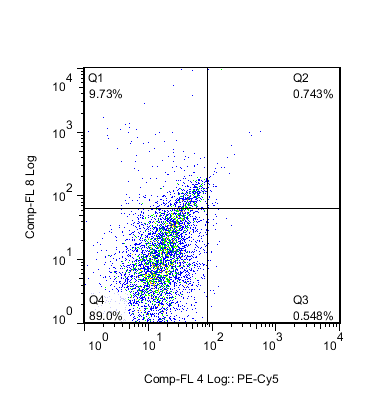
\includegraphics[width=\textwidth]{Figures/Qiagenbeads.png}
\caption{Flow cytometric analysis of lineage depletion using Qiagen beads}
\label{fig:Qiagenbeads}
\end{figure}

%\begin{figure}
	%\begin{subfigure}{\textwidth}
	%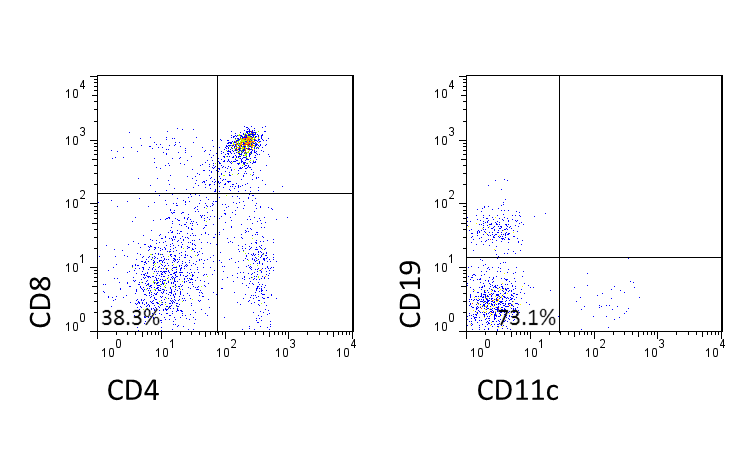
\includegraphics[width=0.8\textwidth]{Figures/1rounddepletion.png}
	%\caption{One round of depletion using Miltenyi lineage depletion beads and columns}
	%\label{subfig:1rounddep}
	%\end{subfigure}
	
	%\begin{subfigure}{0.8\textwidth}
	%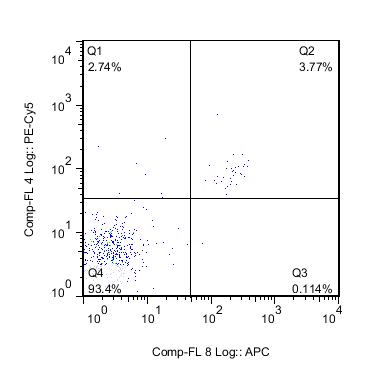
\includegraphics[width=\textwidth]{Figures/2rounddepletion.png}
	%\caption{Two rounds of depletion using Miltenyi lineage depletion beads and columns}
	%\label{subfig:2rounddep}
	%\end{subfigure}
	
	%\begin{subfigure}{0.8\textwidth}
	%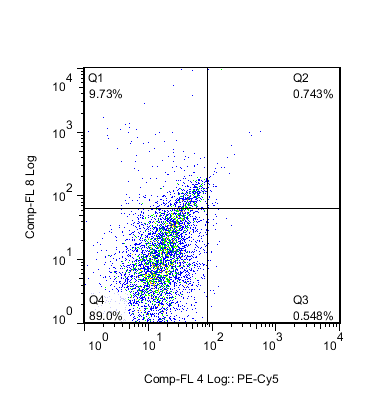
\includegraphics[width=\textwidth] {Figures/Qiagenbeads.png}
	%\caption{Qiagen Beads}
	%\label{subfig:Qiagen}
	%\end{subfigure}
	
%\caption[Optimisation of MACS lineage depletion]{Figure showing the different methods of depletion. 
%Methods for each outlined in \cref{Methods:MACSdepletion}.
%FACS plots gated lymphocytes, single cell CD4\textsuperscript{-}CD8\textsuperscript{-}, then for Miltenyi methods CD19\textsuperscript{-}CD11c\textsuperscript{-} and for Qiagen beads B220\textsuperscript{-}.}
%\end{figure}




%\subsection{BLPs are present in the NOD mouse thymus}

In order to assess the frequency of BLPs present in the thymus of NOD, NOD KO and B6 mice, it was first necessary to establish a suitable gating strategy.
Firstly, data was gated to find the CLP population within the thymus.
For this a lymphocyte and single cell gate was applied then data was gated to anaylse only cells which were Sca-1\textsuperscript{low}c-kit\textsuperscript{low}Flt3\textsuperscript{+}IL-7R$\alpha$\textsuperscript{+}.
From this population, it is then possible to determine which of these cells are BLPs and therefore likely to be B cell committed, depending on their Ly6D expression.
This gating pattern is shown in \cref{subfig:BLPgating}.

When examining the frequencies of BLPs within the thymic CLP population, it appeared that BLPs are present in the thymus of all strains of mice.
However, interestingly, the frequency of BLPs in the thymic CLP population was significantly decreased in the NOD and NOD KO mice compared to the control B6 mice, as shown in \cref{subfig:BLPgraph}.
%This result was unexpected due to the increased thymic B cell population seen in NOD thymi compared to B6 thymi at this age.

The presence of BLPs in the B6 thymus could suggest that they are the normal progenitor for the normal population of thymic B cells seen in nondiabetic animals.
The significant difference in BLP frequencies between NOD mouse strains and control B6 mice may suggest that in NOD mice, thymic B cells originate from an alternative progentitor or developmental pathway.

However, the decreased population of BLPs seen in the NOD mouse could suggest that there may potentially be an alternative mechanism by which B cells increase in the thymus of NOD mice.
With this is mind, other potential B cell development patterns must be explored.
%Interestingly, the analysis gave very inconsistent results for both the WT and KO NOD mice, as shown in \cref{subfig:BLPgraph}.
%The frequencies of each population of cells varied widely over the 3 NOD WT and 4 NOD KO thymi. 
%For example, while the frequencies of Sca-1\textsuperscript{low} and c-kit\textsuperscript{low} cells remained fairly similar for both NOD KO and NOD mice, beyond this point, the percentages of IL-7R$\alpha$\textsuperscript{+}, Flt3\textsuperscript{+} and Ly6D\textsuperscript{+} showed a large amount of variation.
%However, the same was not seen in the B6 control mice.
%These mice showed very consistent frequencies of each population.

%Whilst the data is not hugely useful in determining difference in presence of B cell progenitors, it does suggest that in the B6 mouse, the pattern of development is very well controlled and therefore consistent between mice.
%This contrasts with the mice of NOD background which show huge variablity suggesting that the pattern of development in these mice is much less well controlled.
%This potential lack of control could be contributing to the increase in B cells in the thymus.

%However, despite the variable data from the NOD mice, the data may suggest that actually there are more BLPs present in the B6 mouse compared to the NOD mouse.
%This is surprising due to the significantly increased population of B cells seen in the NOD thymus.


\begin{figure}
	\begin{subfigure}{\textwidth}
	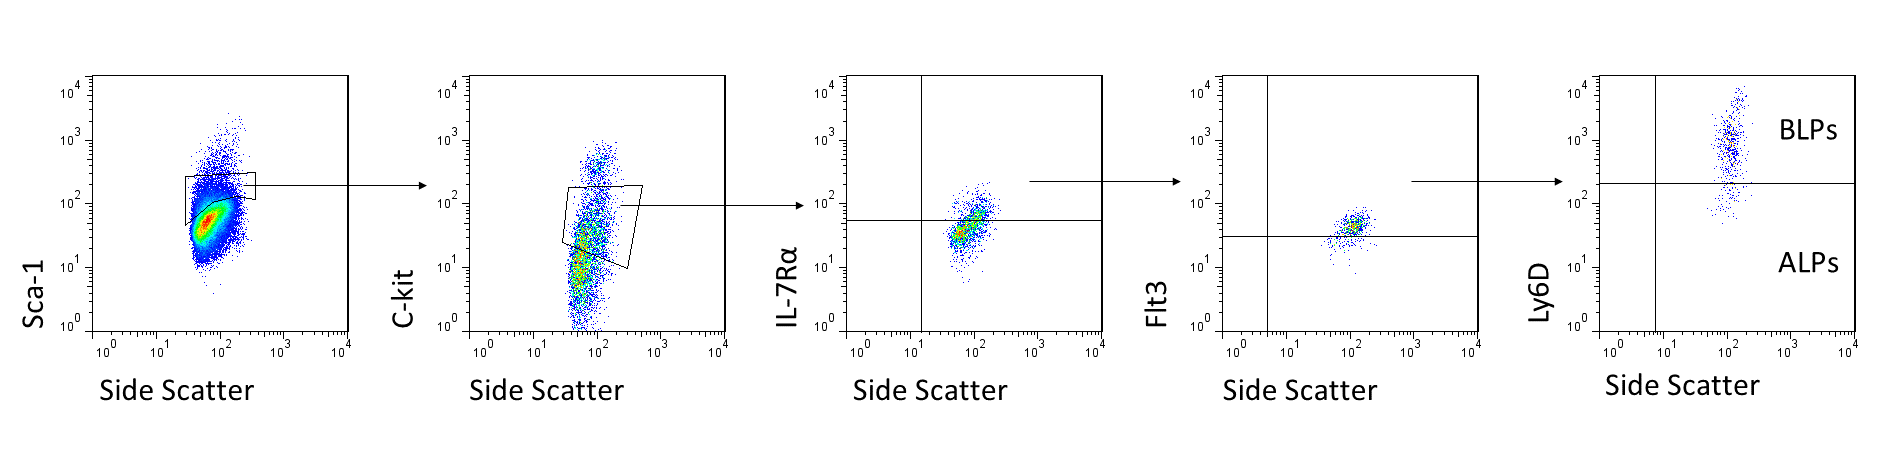
\includegraphics[width=\textwidth]{Figures/BLPgating.png}
	\caption{Gating pattern used to identify BLPs}
	\label{subfig:BLPgating}
	\end{subfigure}
	\begin{subfigure}{\textwidth}
	\centering
	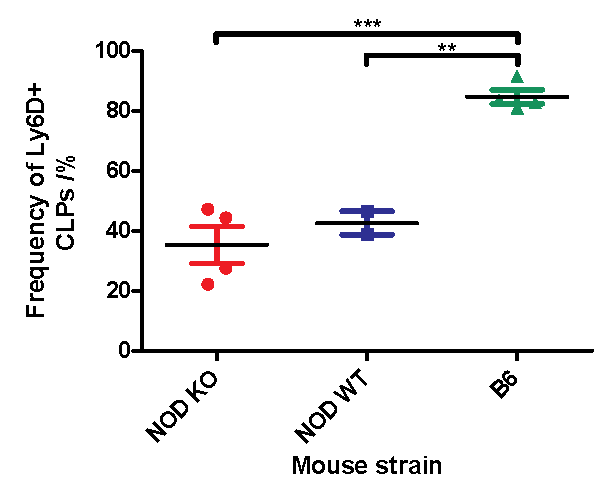
\includegraphics[width=0.6\textwidth]{Figures/Ly6D.pdf}
	\caption{}
	\label{subfig:BLPgraph}
	\end{subfigure}
\caption[BLPs are significantly decreased in the NOD thymus compared to the B6 thymus]{BLPs are present in the NOD thymus. 
Top panel shows gating pattern to look for BLPs in the thymus of mice. Lymphocyte and single cell gate not shown.
Bottom panel shows the frequency of each marker within the population of the previous marker.
One way ANOVA (p=0.0003) and post hoc Tukey's test carried out on Ly6D\textsuperscript{+} population revealing a significantly increased population of BLPs in the B6 mice compared to both NOD and NOD KO thymi.
11 mice were used, all aged 6-8 weeks. 
The experiment was carried out blind to avoid bias. 
NOD WT n=3, NOD KO n=3, B6 n= 4.}
\label{fig:BLPs}
\end{figure}

%Further to this the presence of BLPs in the NOD and NOD KO thymi were compared in older mice, aged 12-13 weeks which correlates with the onset of CTL development and $\beta$ cell destruction \cref{fig:diseasecourse}.
%Unfortunately there were no control B6 mice available at the time, however, it is still possible to suggest whether mature B cells have an effect on the thymic BLP population.
%Mice of this age have a significantly increased thymic B cell population compared to nondiabetic B6 controls \cref{subfig:IncthyBcells}.

%As shown in \cref{fig:olderBLPs}, there is no difference in the frequency of Ly6D\textsuperscript{+} BLPs within the CLP population.
%This may suggest that the action of a mature B cell to increase the pro B cell population in B cell suffcient mice as opposed to B cell deficient mice, is after the BLP stage.

%\begin{figure}
%\centering
%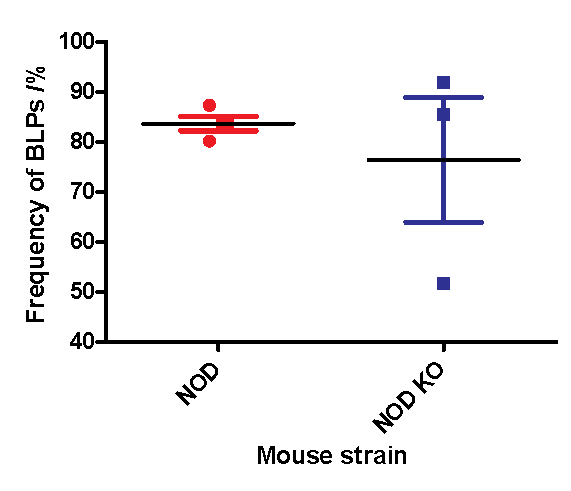
\includegraphics[width=0.6\textwidth]{Figures/NODvKOBLPs.pdf}
%\caption[The frequency of thymic BLPs is the same in both NOD and NOD KO thymi]{Ly6D\textsuperscript{+} BLP presence within the thymic CLP population was assessed by flow cytometry and found to not be statistically significantly different between the NOD and NOD KO thymus. Single cell suspensions were prepared then depleted of CD4, CD8 and CD19 mature cells using Qiagen BioMag goat anti-rat beads. Cells were then incubated with fluorescently-labelled analytic antibodies and assessed by flow cytometry.
%Statistical significance was determined by the Mann Whitney test and the two strains were found to be not statistically significant. NOD n=5, NOD KO n=5.}
%\label{fig:olderBLPs}
%\end{figure}






%\subsection{Conclusion}

%\new{Data to date has so far given evidence that B cells could develop intrathymically.
%I have shown that cells with the phenotype of pro and pre B cells are present in the thymus, suggesting it may be an environment that can support these developing B cells.
%I have also shown that some CD19\textsuperscript{+} cells in the thymus of NOD-RAG-GFP mice are expressing high levels of GFP, suggesting active BcR rearrangement and development.
%It also appears that the thymus is capable of B cell development transcription factor expression.
%This could suggest that the thymus is able to provide an environment conducive to B cell development.
%However, it is necessary to look at B cell development transcription factors quantitatively and then compare this expression to that seen in the B6 thymus.

%There is also evidence to suggest that BLPs are present in the thymus of NOD and B6 mice, though interestingly, it appears that B6 mice may have an increased frequency of BLPs in their thymus compared to the NOD mouse.
%This is not what would be expected due to the significantly increased population of B cells in the NOD thymus.}

\section{Some RAG+ cells in the thymus express B and T cell markers}

B cells normally develop from progenitor BLPs in the bone marrow.
Therefore, initially, BLPs were looked for in the NOD thymus to assess whether or not the normal B cell developmental pattern could be seen in the thymus.
However, following the results suggesting that NOD thymi may have less thymic BLPs compared to the control B6 mice (\cref{subfig:BLPgraph}), an increase in early B cell progenitors is unlikely to account for the increase in thymic B cells in the NOD.
This would suggest that there is an alternative pathway of B cell development in the thymus that is different to the pathway seen in the bone marrow.
%With this in mind, it was noted that a large proportion (>50\%) of GFP\textsuperscript{+}CD19\textsuperscript{+} cells in the NOD thymus, were also CD4\textsuperscript{+}CD8\textsuperscript{+}.
%This was of interest and raised the question as to whether a cell with dual B and T cell markers exist in the NOD thymus and may give rise to bone-fide mature B cells.
%It may be that T cells are able to transform into B cells and that these cells are the midpoint of transition.

\subsection{A large proportion of RAG\textsuperscript{+}CD19\textsuperscript{+} cells in the NOD thymus express CD4 and CD8}

During the course of study, in-depth phenotyping of GFP+ cells in the thymus revealed a surprising finding that CD19+ GFP+ cells expressed CD4 and CD8 T cell markers.
It was decided to follow up this preliminary observation by determining whether there may be a point where thymocytes are not yet fully lineage committed and are expressing markers of both T (CD4, CD8) and B (CD19) cells.

To investigate this, time course flow cytometric studies of the thymus, or control bone marrow, using 4 and 7 week old NOD-RAG-GFP mice were performed.
Mice of 4 and 7 weeks of age were analysed and a representative FACS plot of a 4 week old NOD thymus and bone marrow are shown in \cref{fig:RAGCD19DP}. 
Here, the difference between the thymus \cref{subfig:ThyRAGCD19DP} and bone marrow \cref{subfig:BMRAGCD19DP} is shown.
As shown in \cref{fig:RAGCD19DP}\ref{subfig:ThyRAGCD19DP}, approximately 69.2\% of thymic GFP\textsuperscript{high}CD19\textsuperscript{+} cells also co-expressed CD4 and CD8 molecules.
In contrast, only approximately 5.14\% of GFP\textsuperscript{low}CD19\textsuperscript{+} cells also co-expressed these T cell markers.
This uniqueness for GFP\textsuperscript{high} CD19\textsuperscript{+} cells to co-express CD4 and CD8 molecules was restricted to the thymus, as similar analysis of both the bone marrow and spleen revealed 0.016\% (\cref{fig:RAGCD19DP}\ref{subfig:BMRAGCD19DP}) and 0.38\% (\cref{fig:RAGCD19DP}\ref{subfig:BMRAGCD19DP}) of GFP+CD19+ cells co-express CD4 and CD8 molecules, respectively.


%When GFP\textsuperscript{+}CD19\textsuperscript{+} cells in the NOD thymus were interrogated for CD4 and CD8 expression, as shown in \cref{subfig:ThyRAGCD19DP}, a large percentage of these cells were CD4\textsuperscript{+}CD8\textsuperscript{+}.
%These cells all have a high GFP signal and therefore are actively transcribing the protein, indicating that RAG is also active.
%This suggests that these cells are expressing markers of both T and B cells as well as rearranging a receptor, though it is not possible to tell which one.

%Unfortunately, due to lack of control mice of the correct age, it is not possible to say whether this is a normal pysiological process seen in nondiabetic control mice as well as NOD mice or whether it is unique to the NOD.
%Repetitions of the experiments would need to be carried out with the inclusion of B6 control mice.
%However, due to normal B cell development occurring in the bone marrow, the thymus and bone marrow were compared for presence of RAG\textsuperscript{+}CD19\textsuperscript{+}CD4\textsuperscript{+}CD8\textsuperscript{+} cells and the bone marrow served as a tissue control.

The lack of RAG\textsuperscript{high}CD19\textsuperscript{+}CD4\textsuperscript{+}CD8\textsuperscript{+} cells in the bone marrow suggests it is unlikely that these cells are a normal part of B cell development (\cref{fig:RAGCD19DP}\ref{subfig:BMRAGCD19DP}). %due to the bone marrow being the normal B cell development site.
It is also unlikely that they are a normal part of T cell development as T cell commitment is thought to occur fully in the DN development stage, therefore when developing T cells are still CD4\textsuperscript{-}CD8\textsuperscript{-}.

This suggests that they are thymus specific and it may highlight another abnormality within the NOD thymus that may or may not be related to the increased population of thymic B cells.
It could potentially suggest an alternative mechanism by which B cells are increased in the NOD thymus, and that is that a cell is beginning to commit to the T cell lineage, then at some point receiving a signal which is causing it to begin to switch lineages and start expressing B cell markers.
This potential redifferentiation could explain the existence of both B and T cell markers on the cells. 
However, further research would be required to explore this further.

These RAG\textsuperscript{high}CD19\textsuperscript{+}CD4\textsuperscript{+}CD8\textsuperscript{+} cells are present in the thymus of NOD mice at both 4 and 7 weeks of age and their frequencies \todo{Significance in graph without outlier}  and it was therefore investigated whether or not there was a significant difference in the percentages of these cells between the two age groups, \cref{fig:RAGCD19DP}\ref{BMvThyDPgraph}. 
The bone marrow is also included in the figure as a comparison.
However, the results show that there is no difference in presence of RAG\textsuperscript{high}CD19\textsuperscript{+}CD4\textsuperscript{+}CD8\textsuperscript{+} cells between the two ages. 


Reference figure properly

\begin{figure}	
	\begin{subfigure}{\textwidth}
	\centering
	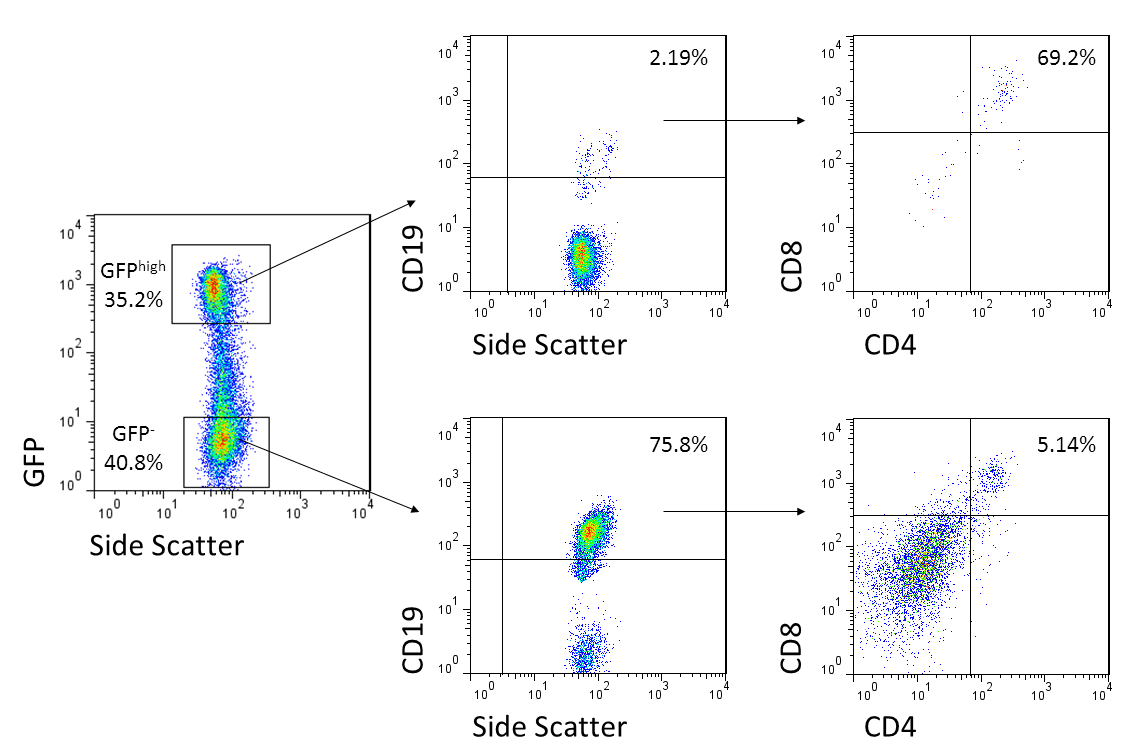
\includegraphics[width=0.85\textwidth]{Figures/GFPCD19CD4CD8.png}
	\caption{Thymus}
	\label{subfig:ThyRAGCD19DP}
	\end{subfigure}
	\begin{subfigure}{0.3\textwidth}
	\centering
	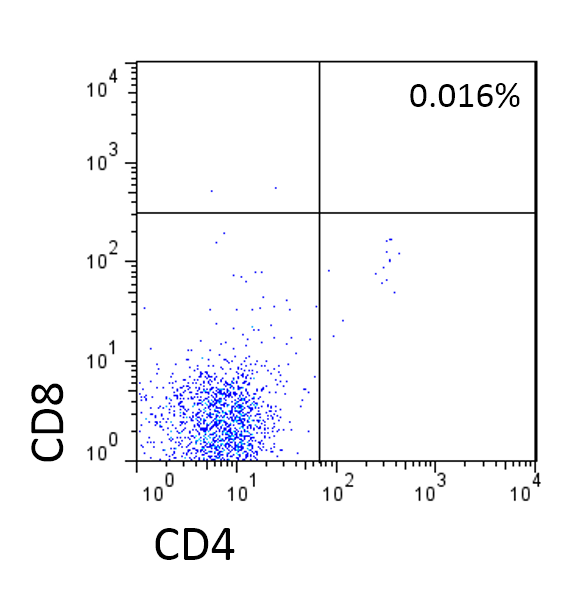
\includegraphics[width=0.9\textwidth]{Figures/BMallposGFPpos.png}
	\caption{Bone marrow GFP+}
	\label{subfig:BMRAGCD19DP}
	\end{subfigure}
	\hfill
	%\begin{subfigure}{0.3\textwidth}
	%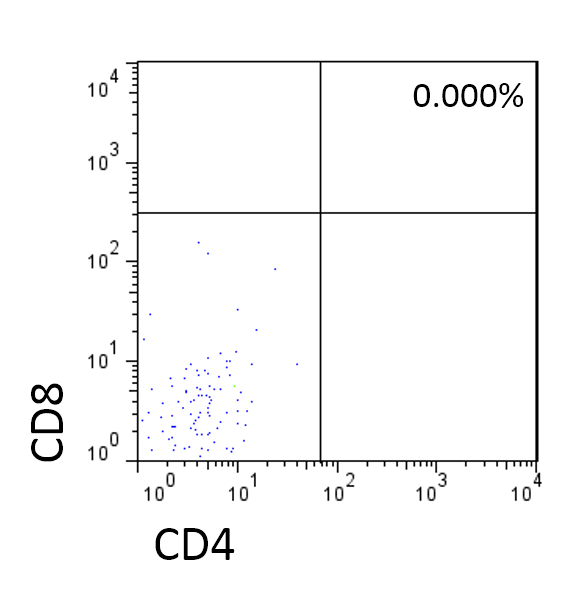
\includegraphics[width=\textwidth]{Figures/BMallposGFPneg.png}
	%\caption{Bone marrow GFP-}
	%\label{subfig:BMRAGCD19DP}
	%\end{subfigure}
	\begin{subfigure}{0.3\textwidth}
	\centering
	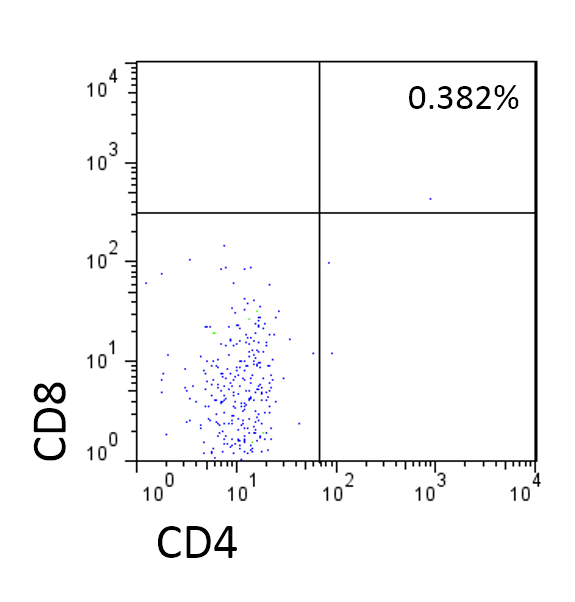
\includegraphics[width=0.9\textwidth]{Figures/SplnallposGFPpos.png}
	\caption{Spleen GFP+}
	\label{subfig:BMRAGCD19DP}
	\end{subfigure}
	\hfill
	%\begin{subfigure}{0.3\textwidth}
	%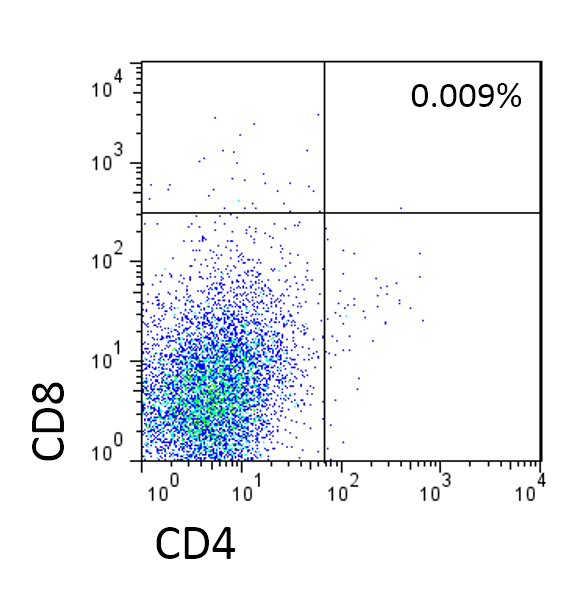
\includegraphics[width=\textwidth]{Figures/SplnallposGFPneg.png}
	%\caption{Spleen GFP-}
	%\label{subfig:BMRAGCD19DP}
	%\end{subfigure}
	\begin{subfigure}{0.3\textwidth}
	\centering
	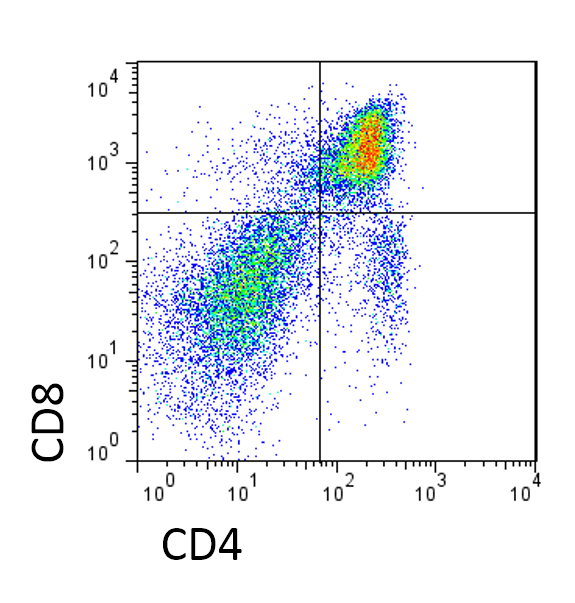
\includegraphics[width=0.9\textwidth]{Figures/Tcellgate.png}
	\caption{T cell gate}
	\label{subfig:Tcellgate}
	\end{subfigure}
	\begin{subfigure}{\textwidth}
	\centering
	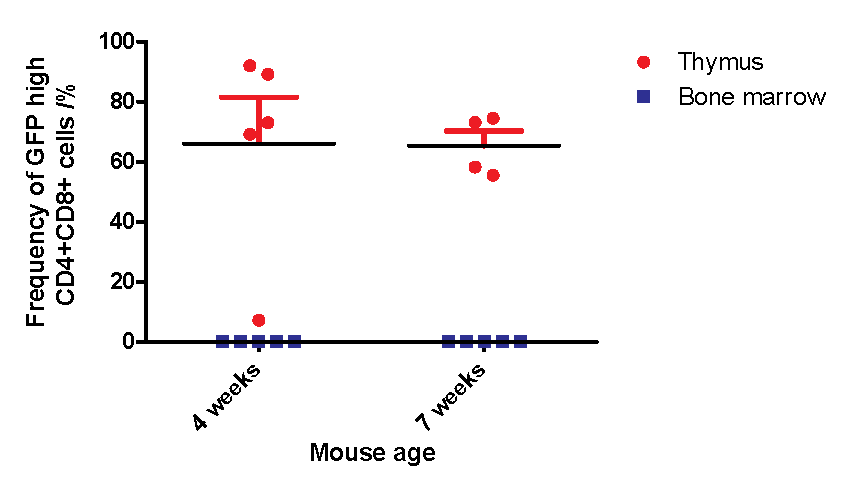
\includegraphics[width=0.7\textwidth]{Figures/RAGCD19CD4CD8ThyBM.pdf}
	\caption{}
	\label{BMvThyDPgraph}
	\end{subfigure}
\caption[There are GFP\textsuperscript{+}CD19\textsuperscript{+}CD4\textsuperscript{+}CD8\textsuperscript{+} cells present in the NOD thymus] {GFP\textsuperscript{+}CD19\textsuperscript{+}CD4\textsuperscript{+}CD8\textsuperscript{+} cells are present in the NOD thymus but not bone marrow or spleen.
Top panel shows representative FACS plot of presence of these cells in the GFP\textsuperscript{high} population in the thymus. A CD19 gate was used on acquisition of data so that 100\% of CD19\textsuperscript{+} cells were acquired with only ~2\% of CD19\textsuperscript{-} cells.
Frequency of CD19\textsuperscript{+}CD4\textsuperscript{+}CD8\textsuperscript{+} cells are much reduced in the GFP\textsuperscript{-} population.
(b) and (c) show the absence of GFP\textsuperscript{+}CD19\textsuperscript{+}CD4\textsuperscript{+}CD8\textsuperscript{+} in the bone marrow and spleen, respectively. Gating used as shown in (a). Data is representative of 5 4 week old NOD-RAG-GFP mice.
(d) shows how the T cell gate was determined. Gated lymphocytes, single cells then while thymus analysed using CD4 and CD8.
Bottom panel shows the lack of GFP\textsuperscript{+}CD19\textsuperscript{+}CD4\textsuperscript{+}CD8\textsuperscript{+} in the bone marrow compared to presence in the thymus. Presence in the thymus is not significantly different between the 2 age groups.
4 week old NOD-RAG-GFP n=5, 7 week old NOD-RAG-GFP n=4.}
\label{fig:RAGCD19DP}
\end{figure}



%Following analysis of the presence of CD19\textsuperscript{+}CD4\textsuperscript{+}CD8\textsuperscript{+} cells on both GFP\textsuperscript{high} and GFP\textsuperscript{low} cells, the expression of IgM on these cells was assessed.
%Interestingly, as shown in \cref{subfig:IgMallpos}, the IgM expression on these cells differed depending on the GFP status.
%CD19\textsuperscript{+}CD4\textsuperscript{+}CD8\textsuperscript{+} cells that were GFP\textsuperscript{high} appeared to have much higher IgM expression compared to those that are GFP\textsuperscript{-}.

%\begin{figure}
%	\begin{subfigure}{\textwidth}
%	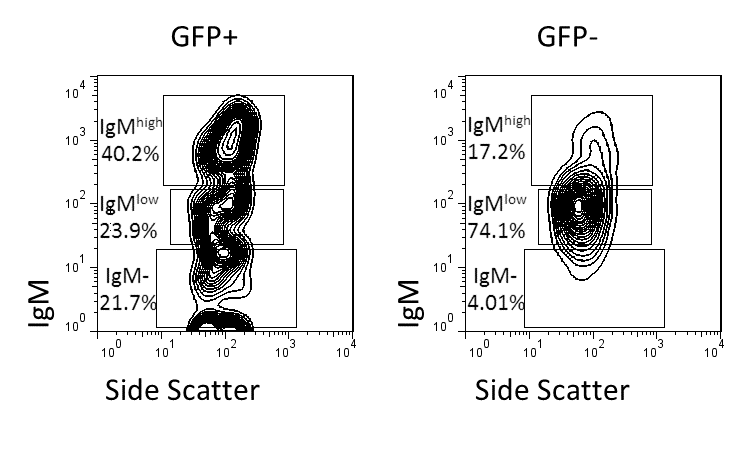
\includegraphics[width=\textwidth]{Figures/IgMallpos.png}
%	\caption{}
%	\label{subfig:IgMallpos}
%	\end{subfigure}
%	\begin{subfigure}{\textwidth}
%	\centering
%	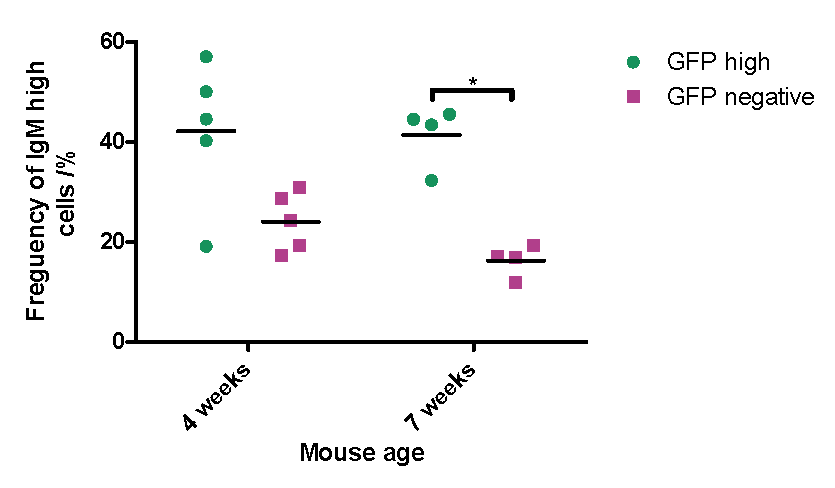
\includegraphics[width=0.7\textwidth]{Figures/IgMhighGFP.pdf}
%	\caption{}
%	\label{subfig:IgMallposgraph}
%	\end{subfigure}
%\caption[IgM expression is higher on CD19\textsuperscript{+}CD4\textsuperscript{+}CD8\textsuperscript{+} cells that are GFP\textsuperscript{high} compared to those that are GFP\textsuperscript{-} in the NOD thymus]{IgM expression is higher on CD19\textsuperscript{+}CD4\textsuperscript{+}CD8\textsuperscript{+} cells that are GFP\textsuperscript{high} compared to those that are GFP\textsuperscript{-} in the NOD thymus.
%Single cell suspensions were prepared and then incubated with analytic flourescently-labelled antibodies for flow cytometric analysis.
%Data was acquired using a CD19 gate whereby 100\% of CD19\textsuperscript{+} cells were acquired along with only approx 2\% of all other cells. For analysis, the data was gated lymphocytes, single cells, GFP\textsuperscript{high} or GFP\textsuperscript{-}, CD19\textsuperscript{+}, CD4\textsuperscript{+}CD8\textsuperscript{+} then analysed according to IgM expression.
%The top panel shows representative plots of IgM expression on CD19\textsuperscript{+}CD4\textsuperscript{+}CD8\textsuperscript{+} that are either GFP\textsuperscript{high} or GFP\textsuperscript{-}.
%The bottom panel shows the frequencies of IgM\textsuperscript{high} cells within either the GFP\textsuperscript{high} or GFP\textsuperscript{-} populations of CD19\textsuperscript{+}CD4\textsuperscript{+}CD8\textsuperscript{+} cells.
%Comparisons of frequencies of IgM\textsuperscript{high} cells between GFP\textsuperscript{high} and GFP\textsuperscript{-} populations at each age were analysed statistically using the Mann Whitney test and found to be statistically significantly different at 7 weeks (p=0.0286) but not 4 weeks of age.
%Gates were set using bone marrow and spleen samples to set levels of IgM.
%n=4/5 NOD-RAG-GFP mice.}
%\label{fig:IgMallpos}
%\end{figure}


\subsection{RAG\textsuperscript{+}IgM\textsuperscript{+}TcR$\beta$\textsuperscript{+} cell presence in the NOD thymus}

While GFP\textsuperscript{+}CD19\textsuperscript{+}CD4\textsuperscript{+}CD8\textsuperscript{+} could potentially be a lymphocyte transitioning from one lineage to another, this is not the only hypothesis.
It may be that a developing T or B cell starts to receive signals which cause it to express markers of both the T and B cell lineage.
If this was the case it was therefore wondered if this cell would continue development and eventually express the receptor for both lineages.
To test this hypothesis, IgM\textsuperscript{+}TcR$\beta$\textsuperscript{+} cells were looked for in the NOD thymus.

%Following the finding of RAG\textsuperscript{+}CD19\textsuperscript{+}CD4\textsuperscript{+}CD8\textsuperscript{+} cells in the thymus, it was then of interest to see if these cells with characteristics of both T and B cells progressed to expressing both a TcR and BcR.
%This would suggest that these cells were somehow continuing further down the developmental pathway and that the Rag was activated and rearranging both a T and B cell receptor.

%To investigate this, the RAG\textsuperscript{+}CD19\textsuperscript{+} were interrogated to see if any expressed both IgM and TcR$\beta$.
As shown in \cref{fig:RAGIgMTcRpos}, it appears that there is a very small population of RAG\textsuperscript{+}IgM\textsuperscript{+}TcR$\beta$\textsuperscript{+} in the thymi of NOD  mice.
None can be seen in control bone marrow preparations. 
the NOD KO which is unsurprising as they are unable to make IgM.
Again, the bone marrow was included as a comparative tissue control.
Data for the bone marrow is not shown as none of the samples showed any RAG\textsuperscript{+}IgM\textsuperscript{+}TcR$\beta$\textsuperscript{+} cells at all (Frequencies = 0\%).

There are some with T and B cell receptors.

This gives the impression that some RAG\textsuperscript{+}CD19\textsuperscript{+}CD4\textsuperscript{+}CD8\textsuperscript{+} cells may progress to displaying both a T and B cell receptor.
This could suggest that these cells are just late at committing to a lineage, or it may be that they are the mid point of either a T or B cell transitioning to the other, or they may be a unique population of thymocyte seen in the NOD thymus.
More extensive investigation into these cells in non diabetes prone mice is warranted.

\todo{Compare NOD thymus and bone marrow rather than NOD and KO}

\begin{figure}
	\begin{subfigure}{\textwidth}
	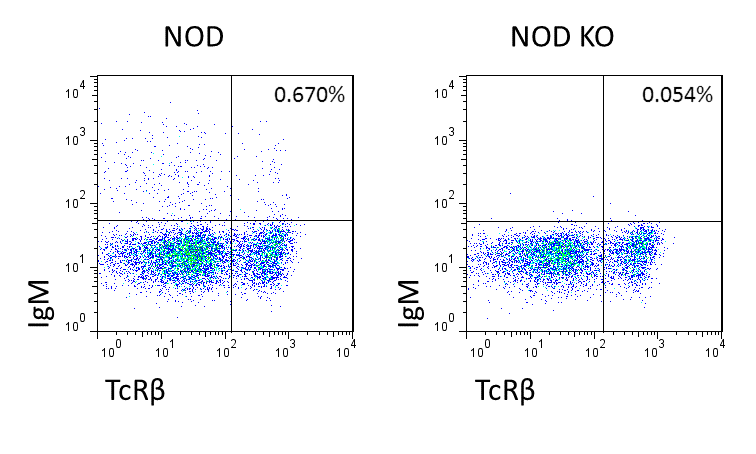
\includegraphics[width=\textwidth]{Figures/NODKOIgMTcR.png}
	\caption{Representative NOD WT and NOD KO thymi looking for RAG+IgM+TcR+ cells. CD19 on acquisition, then lymphocytes, single cells, RAG+ then analysed on IgM and TcR}
	\label{subfig:BMvThyRAGIgMTcR}
	\end{subfigure}
	\begin{subfigure}{\textwidth}
	\centering
	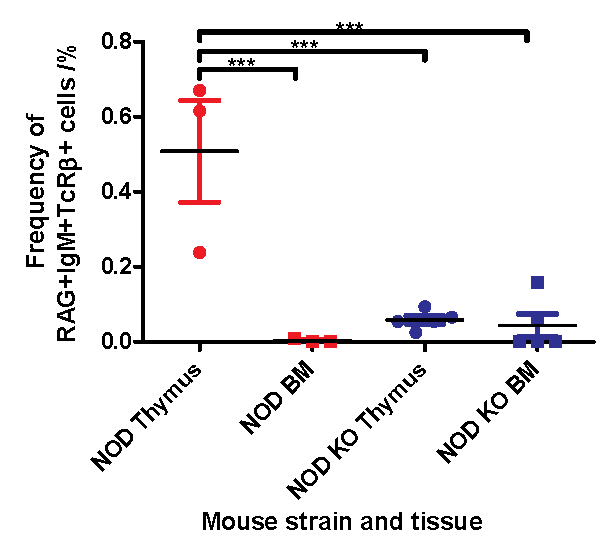
\includegraphics[width=0.7\textwidth]{Figures/IgMTcR.pdf}
	\caption{}
	\label{subfig:IgMTcRposgraph}
	\end{subfigure}
\caption[There is a very small population of IgM\textsuperscript{+}TcR$\beta$\textsuperscript{+} cells in the NOD thymus]{There is a small population of GFP\textsuperscript{+}IgM\textsuperscript{+}TcR$\beta$\textsuperscript{+} cells in the NOD WT thymus. 
Top panel shows a representative NOD WT thymus and NOD KO thymus.
Gated lymphocytes, single cells, GFP\textsuperscript{+} then analysed on IgM and TcR$\beta$ expression.
GFP\textsuperscript{+}IgM\textsuperscript{+}TcR$\beta$\textsuperscript{+} cells are only present in NOD WT and not NOD KO.
Bottom panel shows frequency of GFP\textsuperscript{+}IgM\textsuperscript{+}TcR$\beta$\textsuperscript{+} cells is significantly lower between each strain of mouse. NOD KO < NOD WT < FVB. FVB mice were included as a control.
Results analysed using one-way ANOVA (p=0.0002) and post hoc Tukey's test which revealed a statistically significant differences between the NOD thymus and all other groups.
All mice were RAG-GFP reporter mice and 11 weeks old. NOD WT n=3, NOD KO n=5, FVB n=4.
Thymi and bone marrow from all 12 mice were analysed blind so as not to bias results.}
\label{fig:RAGIgMTcRpos}
\end{figure}



%TcRpos IgMpos for figs - 24.11.14 


%\subsection{IgM\textsuperscript{+}TcRb\textsuperscript{+} cell presence}

%The search for IgM\textsuperscript{+}TcR$\bet$\textsuperscript{+} cells was then widened to exclude Rag\textsuperscript{+} cells and to include thymic and bone marrow tissue from NOD, KO and B6 mice.




%Whether or not there are mature cells present in other tissues in the body that are expressing TcR and IgM was then explored.
%To do this, flow cytometry was carried out on thymic samples from NOD, NOD KO and B6 mice using antibodies specific to TcRb and IgM.
%This time, the spleen was also investigated alongside the thymus and bone marrow to provide another comparison and to widen the search for IgM+TcR+ cells irrelevant of RAG expression.
%Mice of various different ages were investigated and the results are shown in \fig{figure showing TcR+IgM+ cells (or not!)} .
%Isotype controls were also carried out to help with determining whether cells were expressing TcR or IgM or not.
%The data from the isotype controls in shown in \fig{isotype controls}.

%\fig{Spleen, BM, Thymus of IgM+TcR+ cells. NOD v B6 (?Frozen cells)}


%\subsection{Conclusion}

%\new{Whilst there appears to be significant populations of RAG\textsuperscript{high}CD19\textsuperscript{+}CD4\textsuperscript{+}CD8\textsuperscript{+} cells in the NOD thymus, it appears that these cells, on the whole, do not progress to displaying both a TcR and BcR.
%It may, therefore, be that RAG\textsuperscript{high}CD19\textsuperscript{+}CD4\textsuperscript{+}CD8\textsuperscript{+} cells are just B or T cells which are late to commit to a lineage, or it may be that they are the midpoint of a T cell becoming a B cell or vice versa.
%Further investigation, for example culturing of RAG\textsuperscript{high}CD19\textsuperscript{+}CD4\textsuperscript{+}CD8\textsuperscript{+} cells to determine their fate, would be beneficial.}

%\subsection{Conclusion}

%Following the data obtained above, it appears that B cells derived from the thymus don't have a strong preference for migrating back to the thymus following transfer and instead, most migrate to the spleen.
%This could suggest that the function of a thymic B cell is in the spleen, or that thymic B cells do not have the ability to return to the thymus either once they have been removed from the thymus, or following transfer (for example, the necessary features required to home to the thymus may be lost during transfer).

